This chapter presents the technical analysis and specifications underlying the contract management solution. It starts with a benchmark of existing tools and justifies the choice of an Agentic AI-based approach. Then, it reviews the core technologies used, including LLMs, LangChain, and LangGraph. The integration of Langfuse and Tiptap is also introduced. Lastly, the chapter details the system’s functional and non-functional requirements.

\newpage
\fancyhead[R]{\textsc{Chapter 2 - Analysis and Specifications}}
\hypertarget{secondchapter}{}
\section{Comparative Analysis}

This section benchmarks existing contract management and legal automation platforms to highlight their features, strengths, and limitations, providing the rationale for developing our specialized Agentic AI solution.

%% Benchmarking Existing Solutions
\subsection{Benchmarking Existing Solutions}
To evaluate the landscape of intelligent contract management platforms, we analyzed three prominent solutions: PandaDoc, Harvey AI, and DocDraft. Each platform was selected specifically for its focus on contract management and legal automation capabilities.

% PandaDoc
\subsubsection{PandaDoc}
PandaDoc is a comprehensive document automation platform designed to streamline the creation, approval, and management of digital documents, including contracts, proposals, and quotes.\mynewline

\begin{center}
    \centering
    
\includegraphics[width=0.3\textwidth]{Images/PandaDoc_logo.png}
    \captionof{figure}{PandaDoc Logo} \cite{pandadoc_logo}
    \label{fig:pandadoc_logo}
\end{center}

Here are the key features of PandaDoc:
\begin{itemize}
    \item \textbf{Dynamic Contract Templates}: Create and manage reusable templates to ensure consistency and efficiency in document creation.
    \item \textbf{Integrated eSignatures}: Facilitate secure and legally binding electronic signatures within documents. 
    \item \textbf{CRM Integrations}: Seamlessly integrate with platforms like Salesforce and HubSpot to synchronize data and streamline workflows. 
    \item \textbf{Contract Repository}: Centralized storage for contracts, enabling easy access, tracking, and management. 
    \item \textbf{Workflow Automation}: Automate approval processes and notifications to reduce manual intervention and accelerate deal closures. 
\end{itemize}

% Harvey AI
\subsubsection{Harvey AI}
Harvey AI is a generative AI platform designed for legal professionals, enabling advanced legal research, document drafting, and compliance analysis with the support of large language models.\mynewline

\begin{center}
    \centering
    
\includegraphics[width=0.3\textwidth]{Images/harveyai_logo.png}
    \captionof{figure}{Harvey AI Logo} \cite{harveyai_logo}
    \label{fig:harveyai_logo}
\end{center}

Harvey AI’s main functionalities include:
\begin{itemize}
    \item \textbf{AI-Powered Legal Research}: Provides fast, accurate legal research across jurisdictions with references and citations.
    \item \textbf{Document Drafting Automation}: Automates the generation and review of legal documents, reducing time and manual effort.
    \item \textbf{Predictive Analytics}: Leverages historical legal data to forecast case outcomes and support strategic decisions.
    \item \textbf{Secure Document Management}: Ensures safe handling and storage of sensitive legal documents.
    \item \textbf{Customizable AI Models}: Allows tailoring of legal AI agents to specific practice areas, workflows, or jurisdictions.
\end{itemize}

% DocDraftyes
\subsubsection{DocDraft}
DocDraft is an AI-powered contract drafting solution focused on automating the generation, review, and management of legal documents for legal teams and firms.\mynewline

\begin{center}
    \centering
    
\includegraphics[width=0.3\textwidth]{Images/docdraft_logo.png}
    \captionof{figure}{DocDraft Logo} \cite{docdraft_logo}
    \label{fig:docdraft_logo}
\end{center}

DocDraft highlights the following core features:
\begin{itemize}
    \item \textbf{Automated Document Drafting}: Quickly generates contracts and legal documents using intelligent pre-built logic.
    \item \textbf{Clause Library}: Offers a rich repository of standard and customizable clauses for efficient contract assembly.
    \item \textbf{Compliance Checks}: Reviews documents to ensure alignment with relevant laws and regulations.
    \item \textbf{Collaboration Tools}: Enables multiple stakeholders to co-author and comment on documents in real-time.
    \item \textbf{Attorney Matching Service}: Connects users to legal experts for document review and legal consultation.
\end{itemize}

% Comparative Analysis
\subsubsection{Comparative Analysis}
The following table summarizes the key features of the three platforms:\vspace{-0.3cm}

\begin{center}
    \centering
    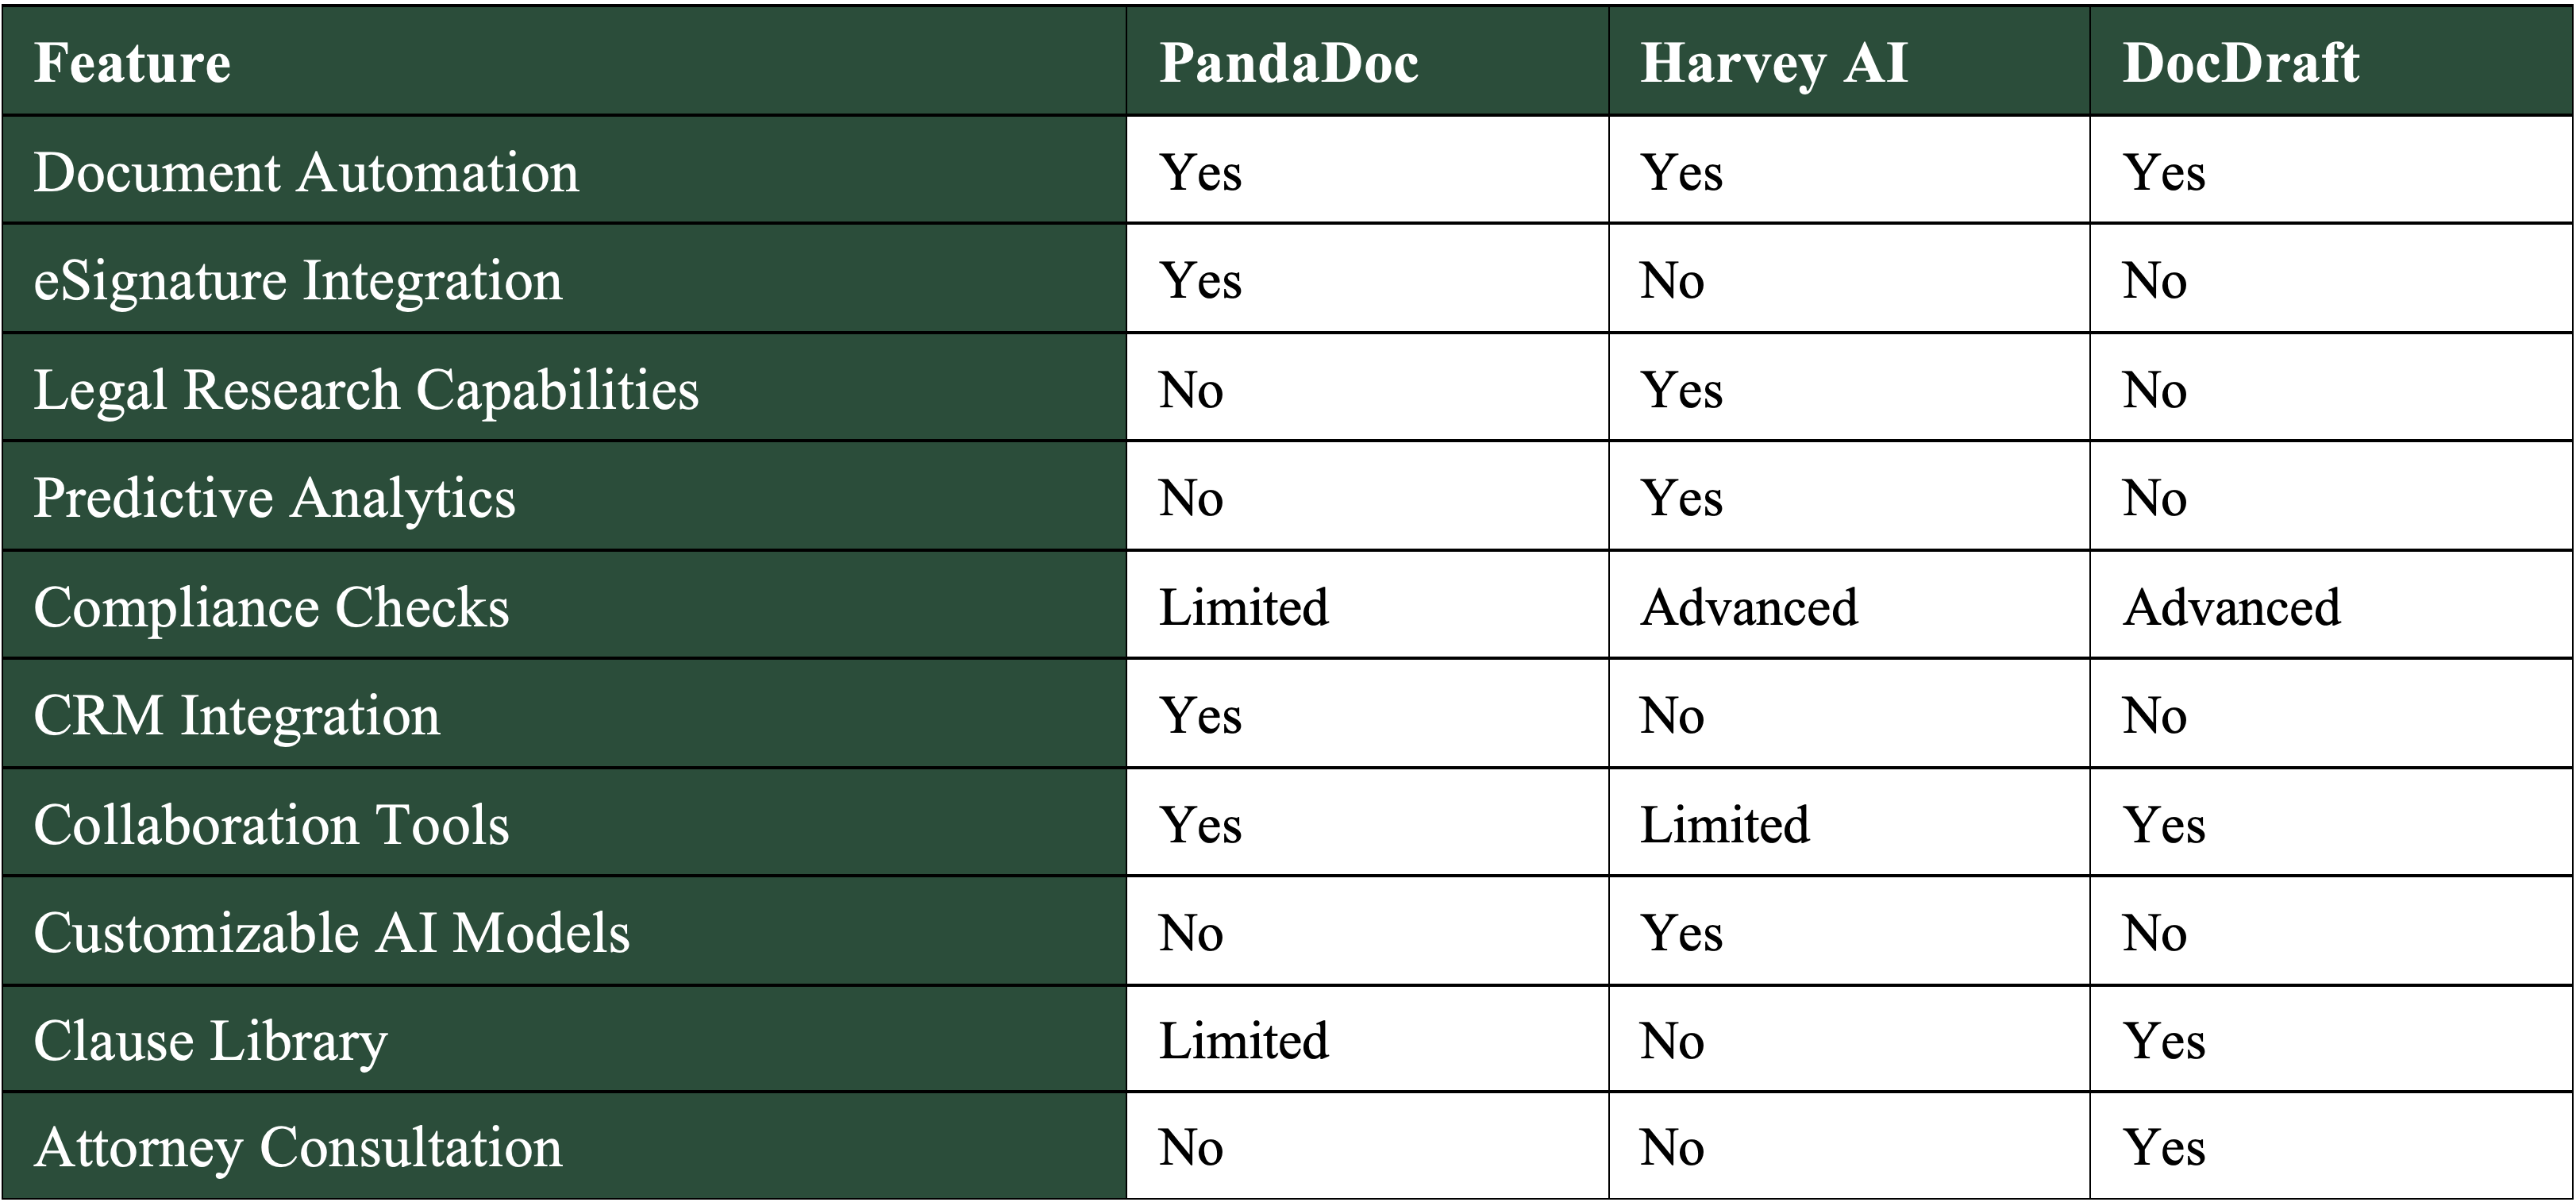
\includegraphics[width=1\textwidth]{Images/Comparison of Contract Management and Legal AI Platforms.png}
    \captionof{table}{Imperative vs. Agentic Approach Comparison}
    \label{tab:comparison_legal_platforms}
\end{center}

% Why We Chose to Build a New Solution
\subsection{Why We Chose to Build a New Solution}
The comparative study clearly revealed that existing contract management platforms were not sufficient to meet our needs. Most tools offer limited automation capabilities and lack the flexibility required for complex legal workflows. Additionally, their inability to support deep integration with enterprise systems, limited orchestration features, and lack of control over agent behavior made them unsuitable for large-scale deployment.\mynewline

To overcome these limitations, we chose to develop a custom solution based on agentic AI. This approach allows us to build a modular, scalable system capable of automating contract drafting, compliance checks, and collaboration, all within a secure and integrated enterprise environment. The goal was not only to improve current processes, but also to lay a solid foundation for future legal automation use cases.\mynewline

To achieve this, we evaluated two principal approaches for building intelligent automation solutions: the traditional imperative approach and the more advanced declarative (agentic) approach. The imperative approach relies on explicit instructions and manual intervention, while the declarative approach leverages autonomous AI agents capable of dynamically adapting to tasks and goals.\mynewline

A detailed comparison of these two methodologies, highlighting the specific advantages of the agentic approach, is presented in Table~\ref{tab:imperative_vs_declarative}. This comparison clearly demonstrates why the agentic (declarative) methodology is more aligned with our requirements and vision, guiding our architectural direction.

\begin{center}
    \centering
    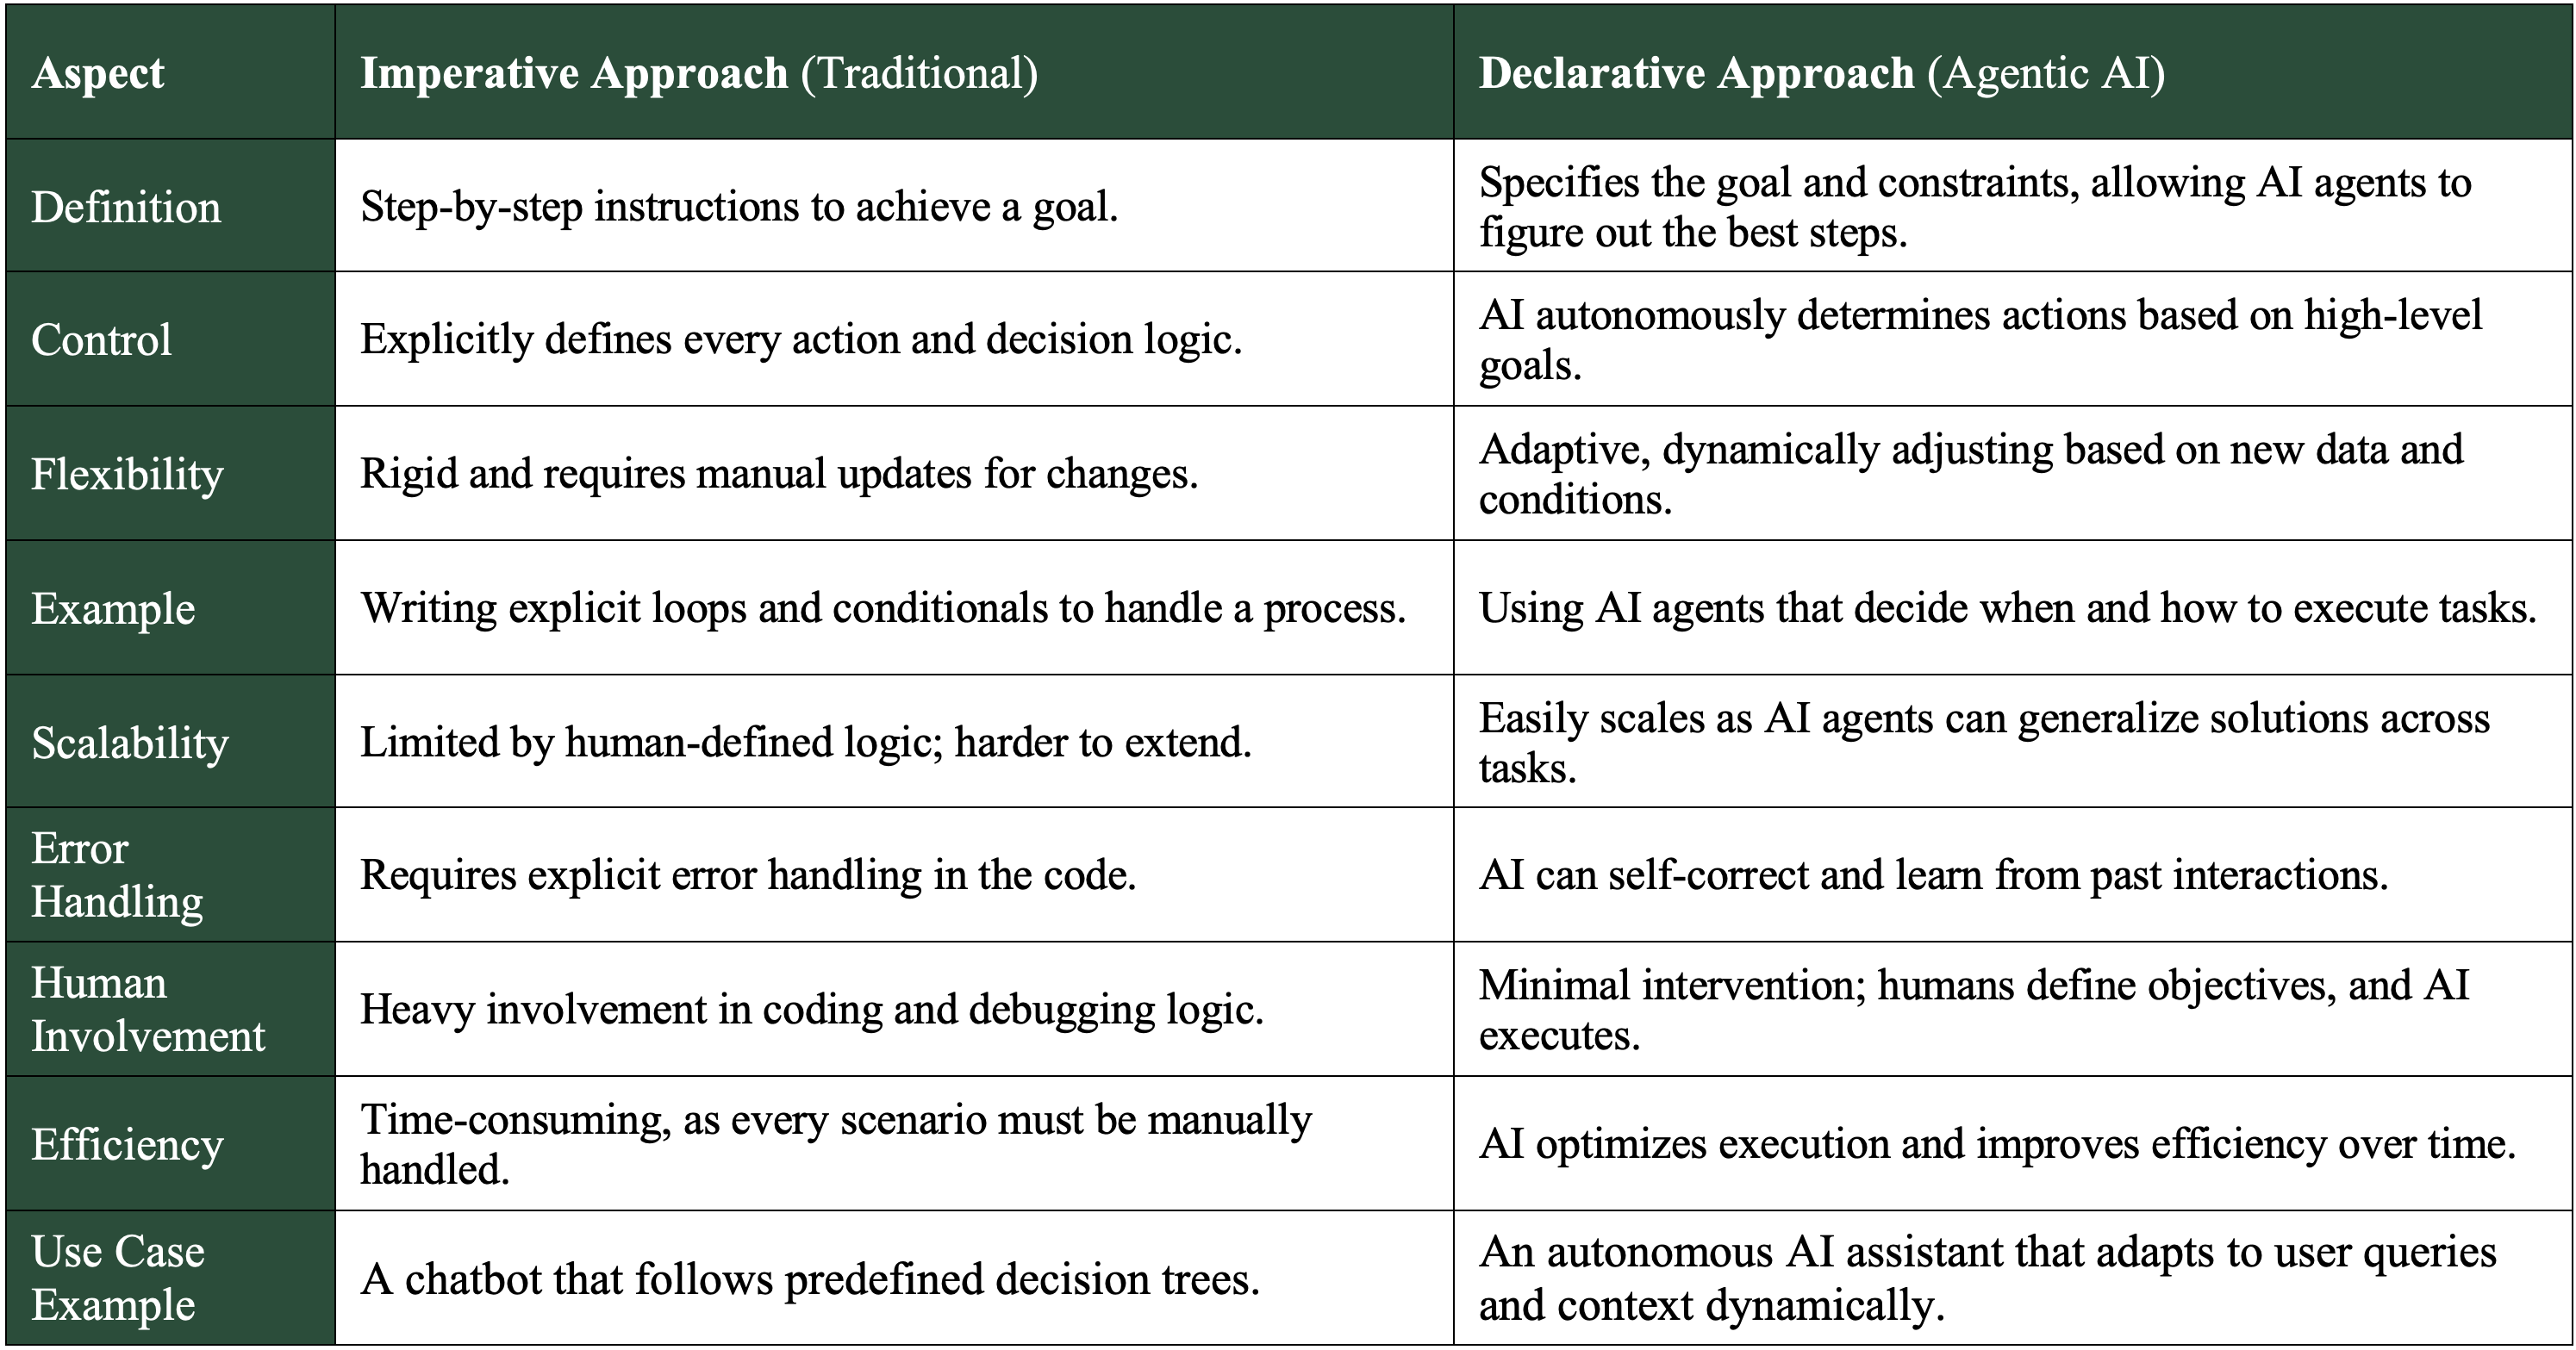
\includegraphics[width=1\textwidth]{Images/Imperative vs. Agentic Approach Comparison.png}
    \captionof{table}{Imperative vs. Agentic Approach Comparison}
    \label{tab:imperative_vs_declarative}
\end{center}


% Technical Background
\section{Technical Background}
This section provides an overview of key technologies enabling the platform's intelligent functionalities.

% Large Language Models (LLMs)
\subsection{Large Language Models (LLMs)}

\subsubsection{Overview}
Large Language Models (LLMs) have revolutionized natural language processing through transformer-based architectures, extensive computational resources, and vast datasets, achieving near-human performance in various linguistic tasks.

\begin{center}
    \centering
    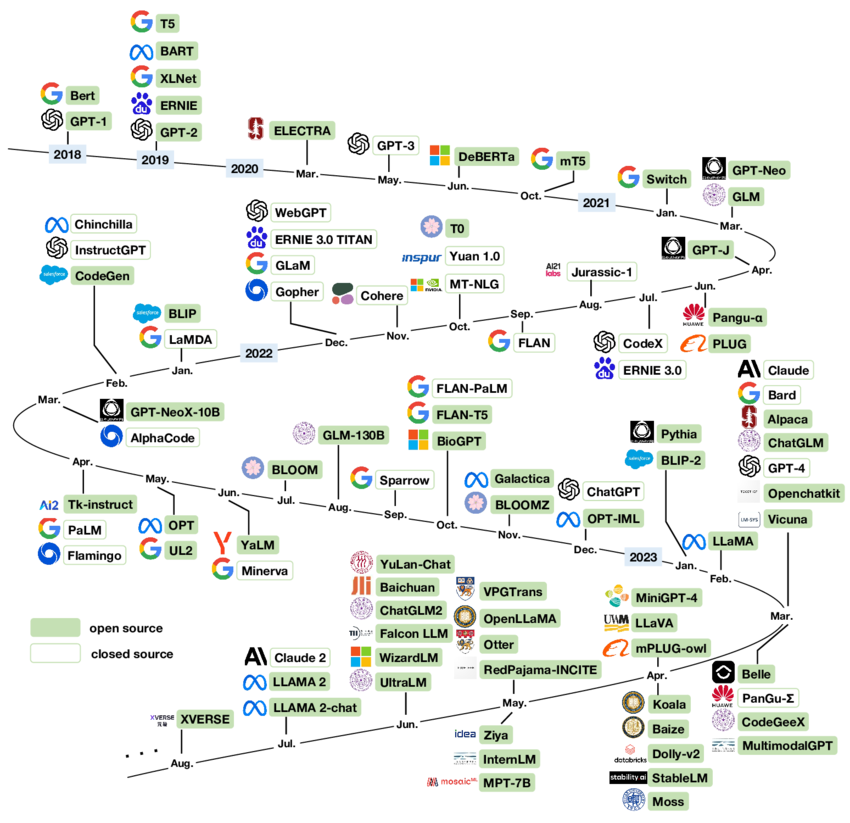
\includegraphics[width=0.9\textwidth]{Images/evolution chronologic LLM.png}
    \captionof{figure}{Chronological Evolution of Large Language Models (LLMs)} \cite{llmEvolution}
    \label{fig:llmEvolution}
\end{center}

\subsubsection{Capabilities and Emergent Properties}
Large Language Models have significantly evolved, exhibiting capabilities such as reasoning, decision-making, and in-context learning, often emerging spontaneously at scale rather than through explicit programming or training. These emergent properties enable LLMs to effectively generalize across diverse tasks without extensive task-specific data, highlighting their robust adaptability. Techniques such as fine-tuning and prompt engineering further enhance model alignment, ensuring outputs align closely with user intents and expectations.\mynewline

LLMs’ adaptability and versatility have found applications in various sectors including healthcare, finance, legal operations, and customer service, underscoring their transformative potential across industries.

\subsubsection{Challenges and Limitations}
Despite these advancements, LLM deployment is constrained by several critical limitations. Key challenges include:

\begin{itemize}
    \item \textbf{Computational Cost and Efficiency}: The resource-intensive nature of LLM training and inference demands considerable computational power, resulting in high operational costs.
    \item \textbf{Input Size Constraints}: Current LLM architectures typically handle context windows of up to 128k tokens, limiting their ability to directly process large-scale data sources comprising millions of tokens.
    \item \textbf{Inference Speed and Latency}: Longer inputs proportionally increase inference time and computational demands, challenging real-time or large-scale applications.
    \item \textbf{Ethical and Bias Considerations}: Models may inadvertently propagate biases present in training data or generate misleading and potentially harmful outputs, necessitating robust ethical oversight.
\end{itemize}

\subsubsection{Future Directions}
Addressing these constraints has become an active area of research. Innovations in model compression techniques, such as pruning, quantization, and distillation, aim to enhance efficiency and accessibility of LLMs. Moreover, emerging architectures and retrieval-augmented generation methods offer promising approaches for handling extensive datasets and large input contexts effectively.

Future advancements are expected to mitigate current limitations, further unlocking the full potential of Large Language Models across diverse, complex applications.

% Agentic AI
\subsection{Agentic AI}

\subsubsection{Overview}
Agentic AI represents a significant evolution in artificial intelligence, transitioning from reactive systems to proactive, autonomous entities capable of setting goals, making decisions, and adapting to dynamic environments. Unlike traditional AI agents that operate within predefined parameters, Agentic AI systems exhibit autonomy, learning, and adaptability, enabling them to handle complex, multi-step tasks with minimal human intervention.

\begin{center}
    \centering
    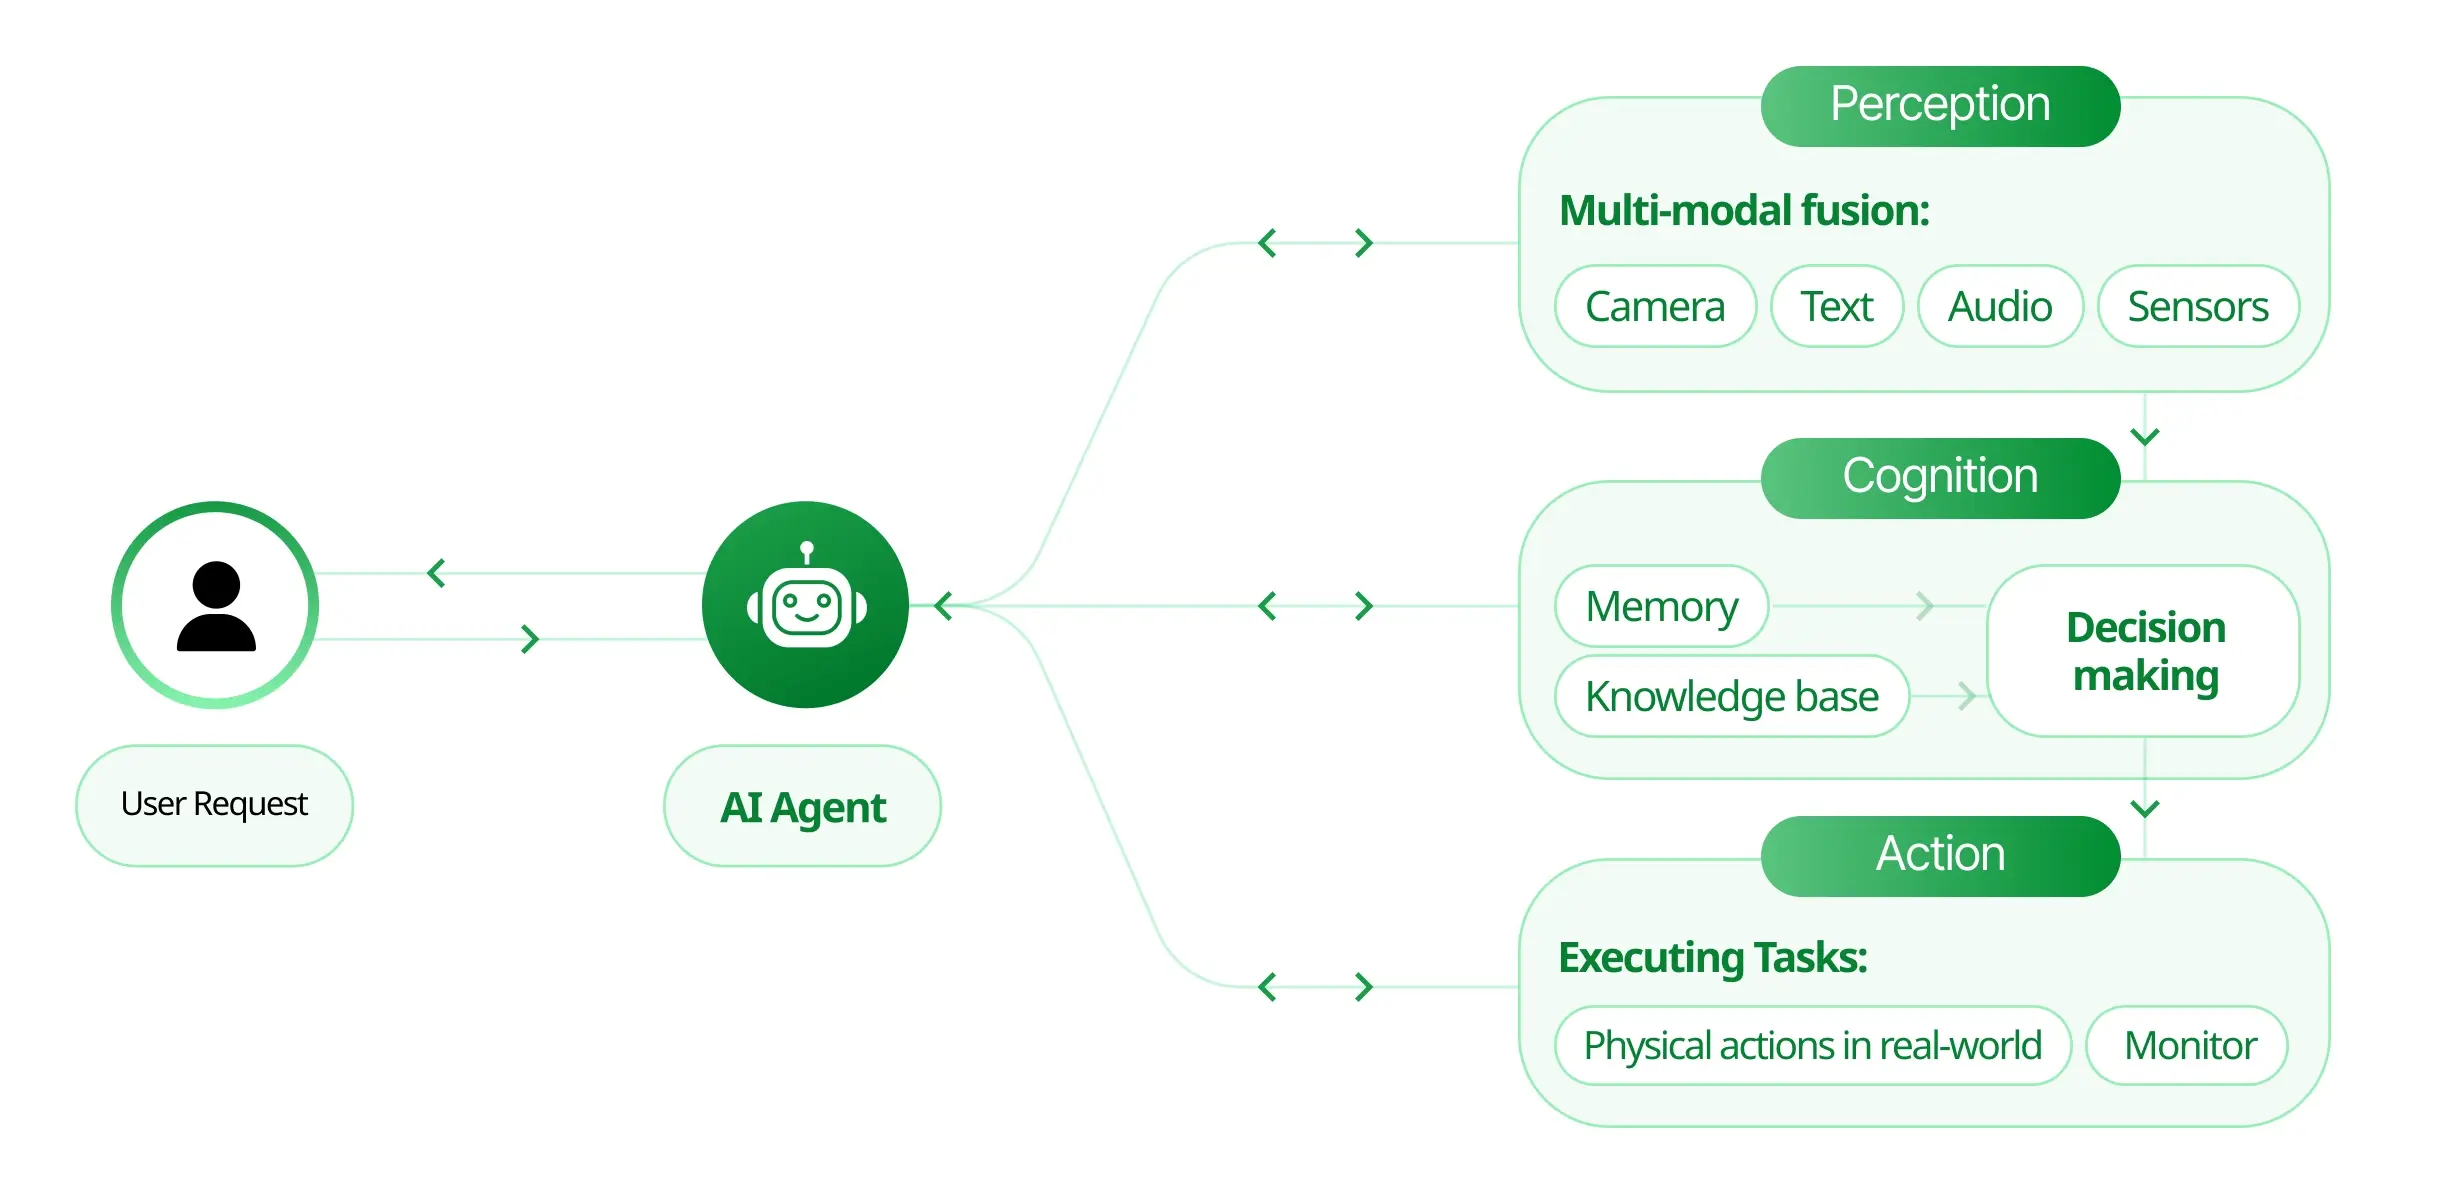
\includegraphics[width=0.9\textwidth]{Images/agentic_ai_architecture.png}
    \captionof{figure}{Agentic AI System Architecture} \cite{agenticAIArchitecture}
    \label{fig:agentic_ai_architecture}
\end{center}

\subsubsection{Core Characteristics}
Agentic AI systems are distinguished by several key features:

\begin{itemize}
    \item \textbf{Autonomy}: They operate independently, making decisions without continuous human oversight.
    \item \textbf{Goal-Oriented Behavior}: These systems can set, pursue, and adjust goals based on environmental feedback.
    \item \textbf{Adaptability}: Agentic AI learns from experiences, refining its strategies to improve performance over time.
    \item \textbf{Complex Decision-Making}: They evaluate multiple options and potential outcomes to make informed decisions.
    \item \textbf{Collaboration}: Agentic AI can coordinate with other agents or systems to achieve shared objectives.
\end{itemize}

\subsubsection{Agentic AI vs. Generative AI}
While both Agentic AI and Generative AI leverage advanced machine learning techniques, their functionalities differ significantly:

\begin{itemize}
    \item \textbf{Generative AI}: Focuses on creating content (text, images, etc.) based on input data, operating primarily in a reactive manner.
    \item \textbf{Agentic AI}: Emphasizes autonomous decision-making and goal pursuit, enabling proactive interactions with the environment.
\end{itemize}

\begin{center}
    \centering
    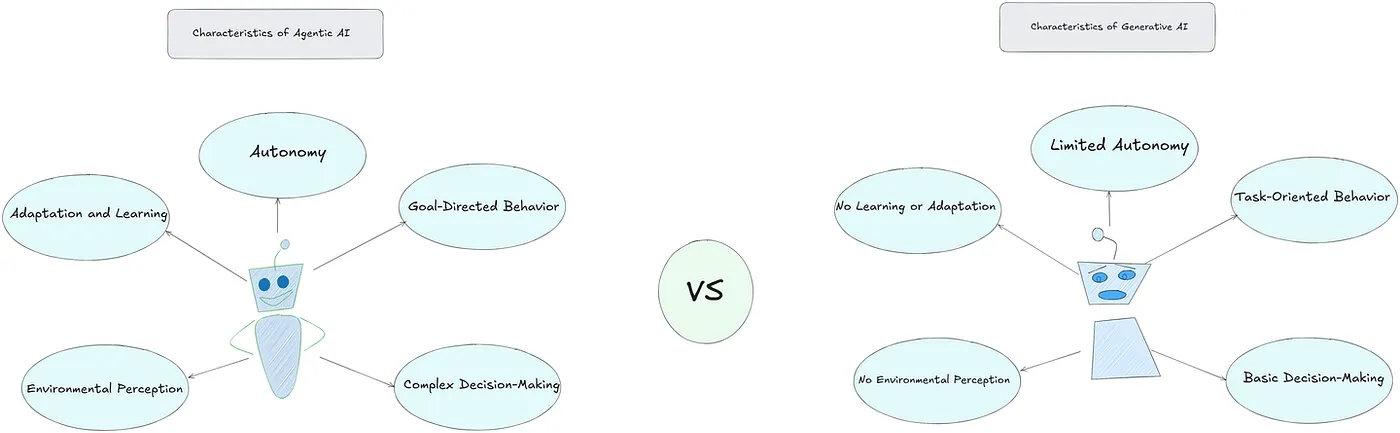
\includegraphics[width=1\textwidth]{Images/agentic_vs_generative_ai.png}
    \captionof{figure}{Comparison Between Agentic AI and Generative AI} \cite{agentic_vs_generative_ai}
    \label{fig:agentic_vs_generative_ai}
\end{center}

\subsubsection{Multi-Agent Systems}
Agentic AI often operates within multi-agent systems, where multiple autonomous agents collaborate to solve complex problems. These systems benefit from:

\begin{itemize}
    \item \textbf{Specialization}: Agents can focus on specific tasks, enhancing efficiency.
    \item \textbf{Scalability}: Systems can be expanded by adding more agents to handle increased complexity.
    \item \textbf{Robustness}: Collaboration among agents can compensate for individual agent failures or limitations.
\end{itemize}

\begin{center}
    \centering
    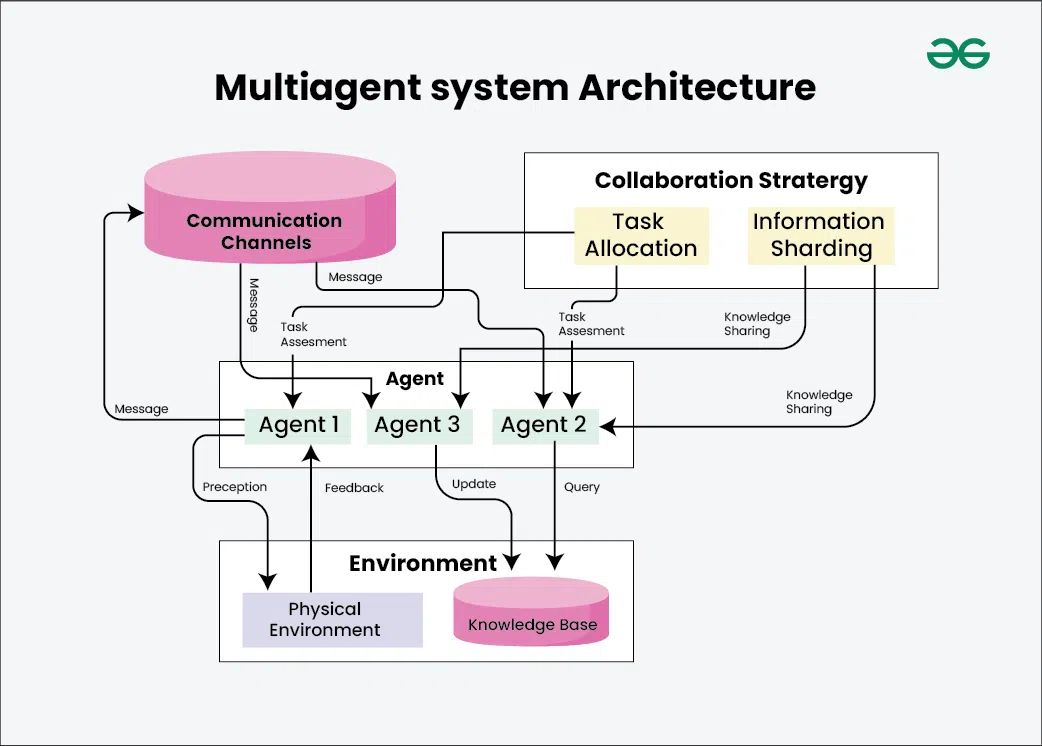
\includegraphics[width=0.9\textwidth]{Images/multi_agent_system.png}
    \captionof{figure}{Multi-Agent System Collaboration} \cite{multi_agent_system}
    \label{fig:multi_agent_system}
\end{center}

\subsubsection{Challenges and Future Directions}
Despite its potential, Agentic AI faces several challenges:

\begin{itemize}
    \item \textbf{Ethical Considerations}: Ensuring decisions align with human values and societal norms.
    \item \textbf{Transparency}: Making decision-making processes understandable to users.
    \item \textbf{Security}: Protecting systems from malicious manipulation or unintended behaviors.
    \item \textbf{Integration}: Seamlessly incorporating Agentic AI into existing infrastructures.
\end{itemize}

Ongoing research aims to address these challenges, focusing on developing frameworks for ethical AI, enhancing interpretability, and establishing standards for safe deployment.

% LangChain and LangGraph
\subsection{LangChain and LangGraph}

\subsubsection{Overview}
LangChain and LangGraph are complementary frameworks designed to facilitate the development of applications powered by Large Language Models (LLMs). While LangChain provides a modular approach to constructing sequential workflows, LangGraph introduces a graph-based paradigm, enabling the creation of complex, dynamic, and stateful AI systems.

\subsubsection{LangChain: Modular Workflow Construction}
LangChain is an open-source framework that simplifies the integration of LLMs into applications by allowing developers to build chains—sequences of calls to LLMs and other utilities. Its modular design supports the composition of various components such as prompt templates, memory modules, and tool integrations. This structure is particularly effective for tasks that follow a linear progression, such as document summarization, question answering, and conversational agents.

\begin{center}
    \centering
    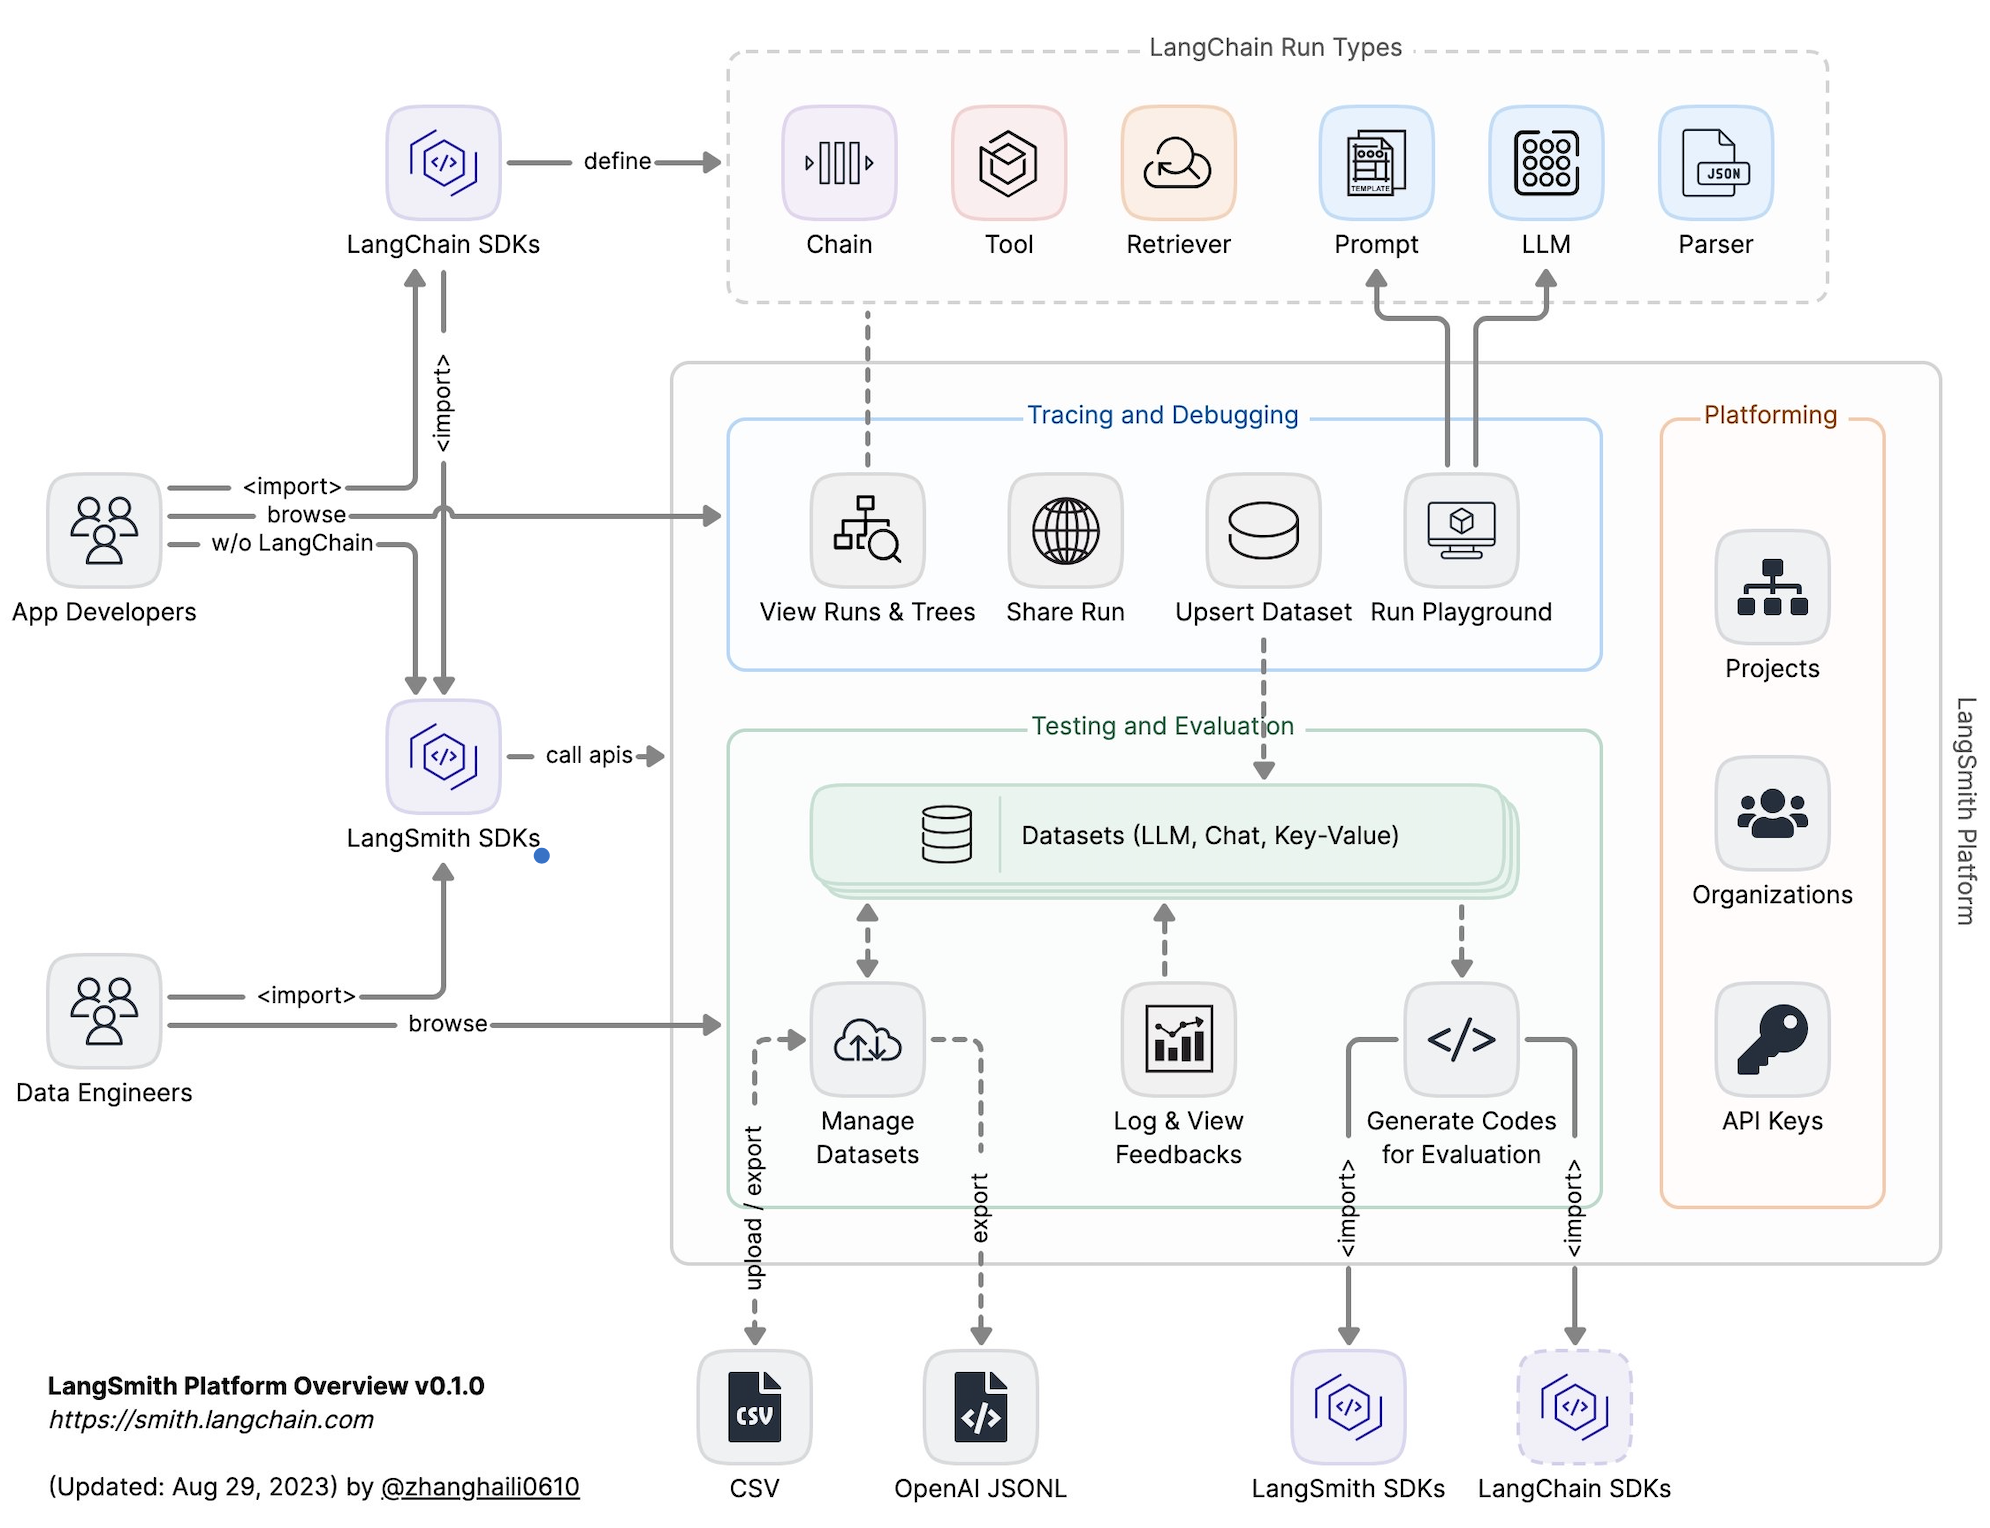
\includegraphics[width=0.9\textwidth]{Images/Langchain Architecture.png}
    \captionof{figure}{LangChain Architecture} \cite{langchainArchitecture}
    \label{fig:langchain_architecture}
\end{center}

Key features of LangChain include:
\begin{itemize}
    \item \textbf{Prompt Templates}: Facilitate the creation of dynamic prompts for LLMs.
    \item \textbf{Chains}: Enable the linking of multiple components to form a cohesive workflow.
    \item \textbf{Agents}: Allow for decision-making capabilities by selecting appropriate actions based on user input.
    \item \textbf{Memory}: Maintain context across interactions to support stateful conversations.
\end{itemize}

\subsubsection{LangGraph: Graph-Based Workflow Orchestration}
Building upon the foundations of LangChain, LangGraph introduces a graph-based approach to workflow orchestration, allowing for the modeling of complex, non-linear, and cyclical processes. In LangGraph, workflows are represented as directed graphs comprising nodes (representing operations or agents) and edges (defining the flow between nodes). This structure is particularly advantageous for applications requiring iterative processing, conditional branching, and multi-agent coordination.

\begin{center}
    \centering
    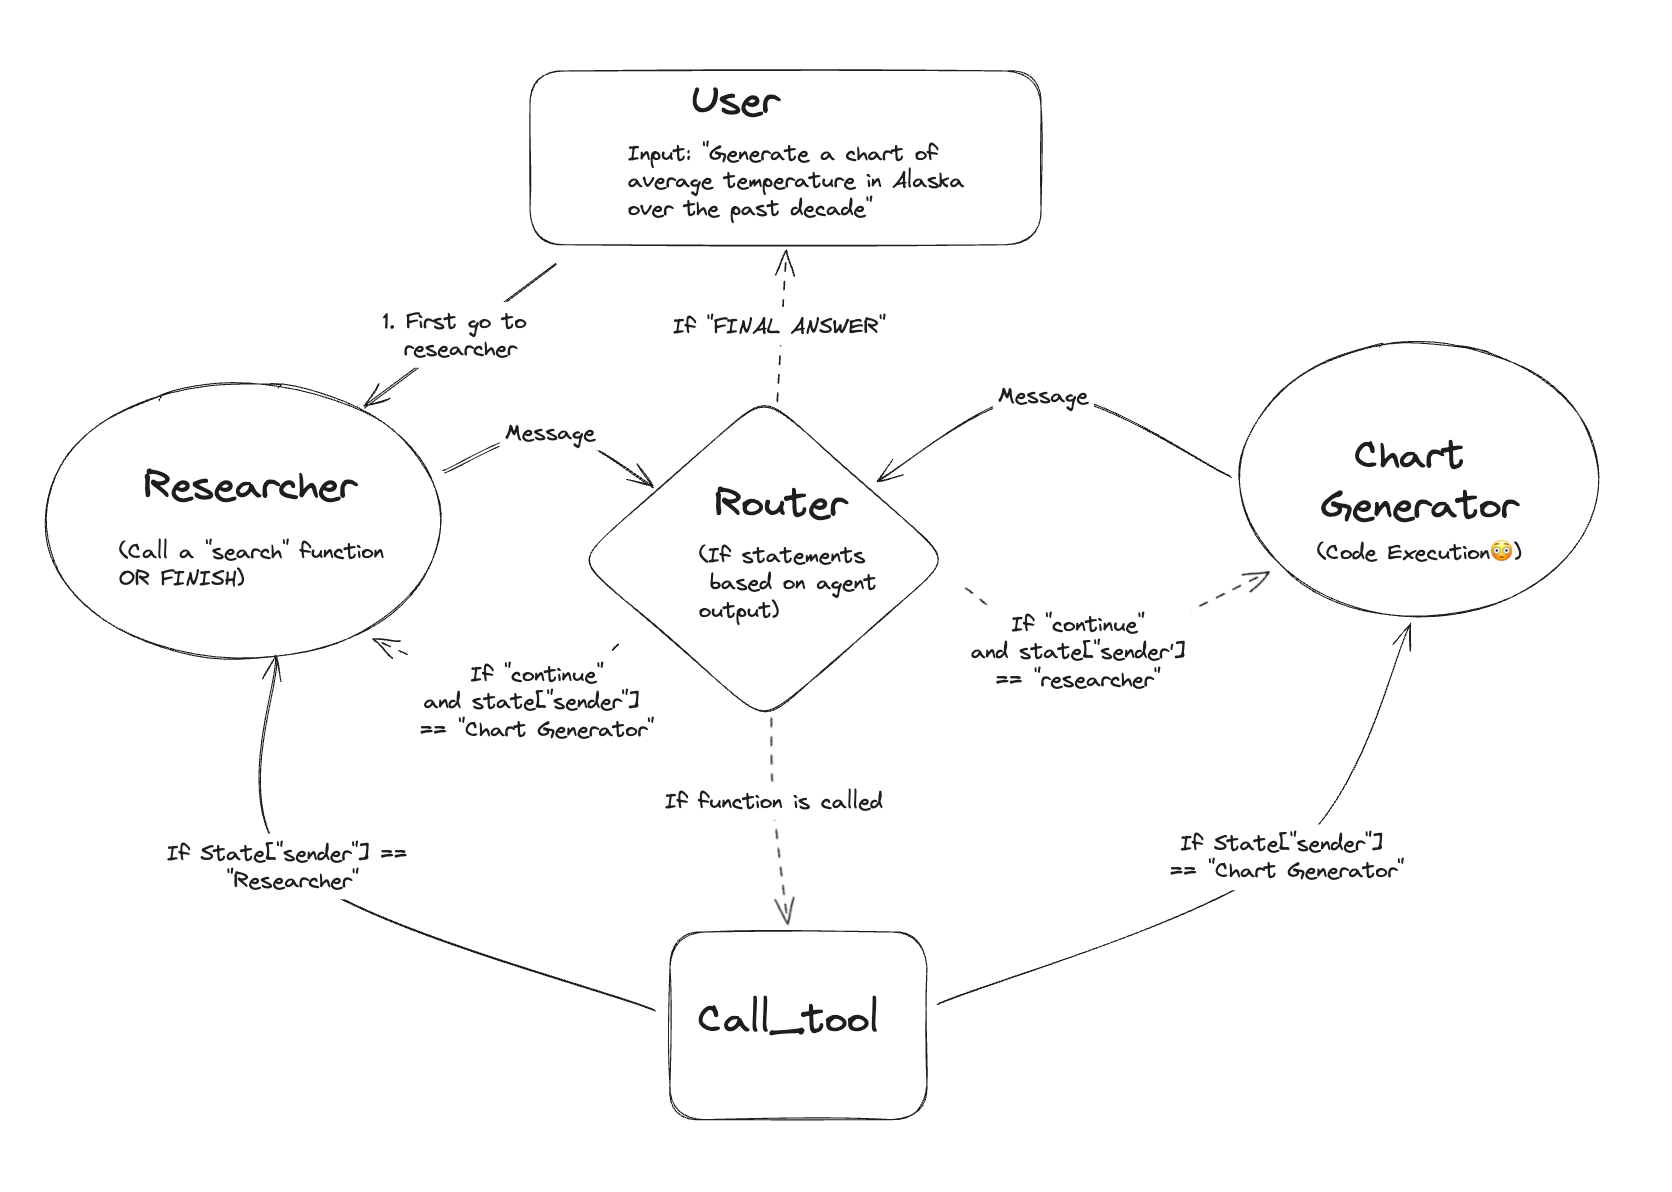
\includegraphics[width=0.9\textwidth]{Images/langgraph_mutil_agent.png}
    \captionof{figure}{LangGraph: Multi-Agent Workflows} \cite{langgraphMultiAgent}
    \label{fig:langgraph_multi_agent}
\end{center}

Notable capabilities of LangGraph include:
\begin{itemize}
    \item \textbf{Cyclic Workflows}: Support for loops and iterative processes within workflows.
    \item \textbf{Conditional Routing}: Dynamic decision-making to determine the next node based on runtime conditions.
    \item \textbf{State Management}: Persistent tracking of the system’s state throughout the workflow execution.
    \item \textbf{Multi-Agent Collaboration}: Facilitation of interactions between multiple agents, each with specialized roles.
\end{itemize}

\subsubsection{Comparative Analysis}
LangChain and LangGraph streamline the development of LLM-powered applications but address varying complexity levels. LangChain is optimal for linear workflows with straightforward tasks and limited iterative processes. In contrast, LangGraph’s dynamic, graph-based structure efficiently manages more intricate workflows involving conditional logic, iterative loops, and robust multi-agent coordination.

\begin{center}
    \centering
    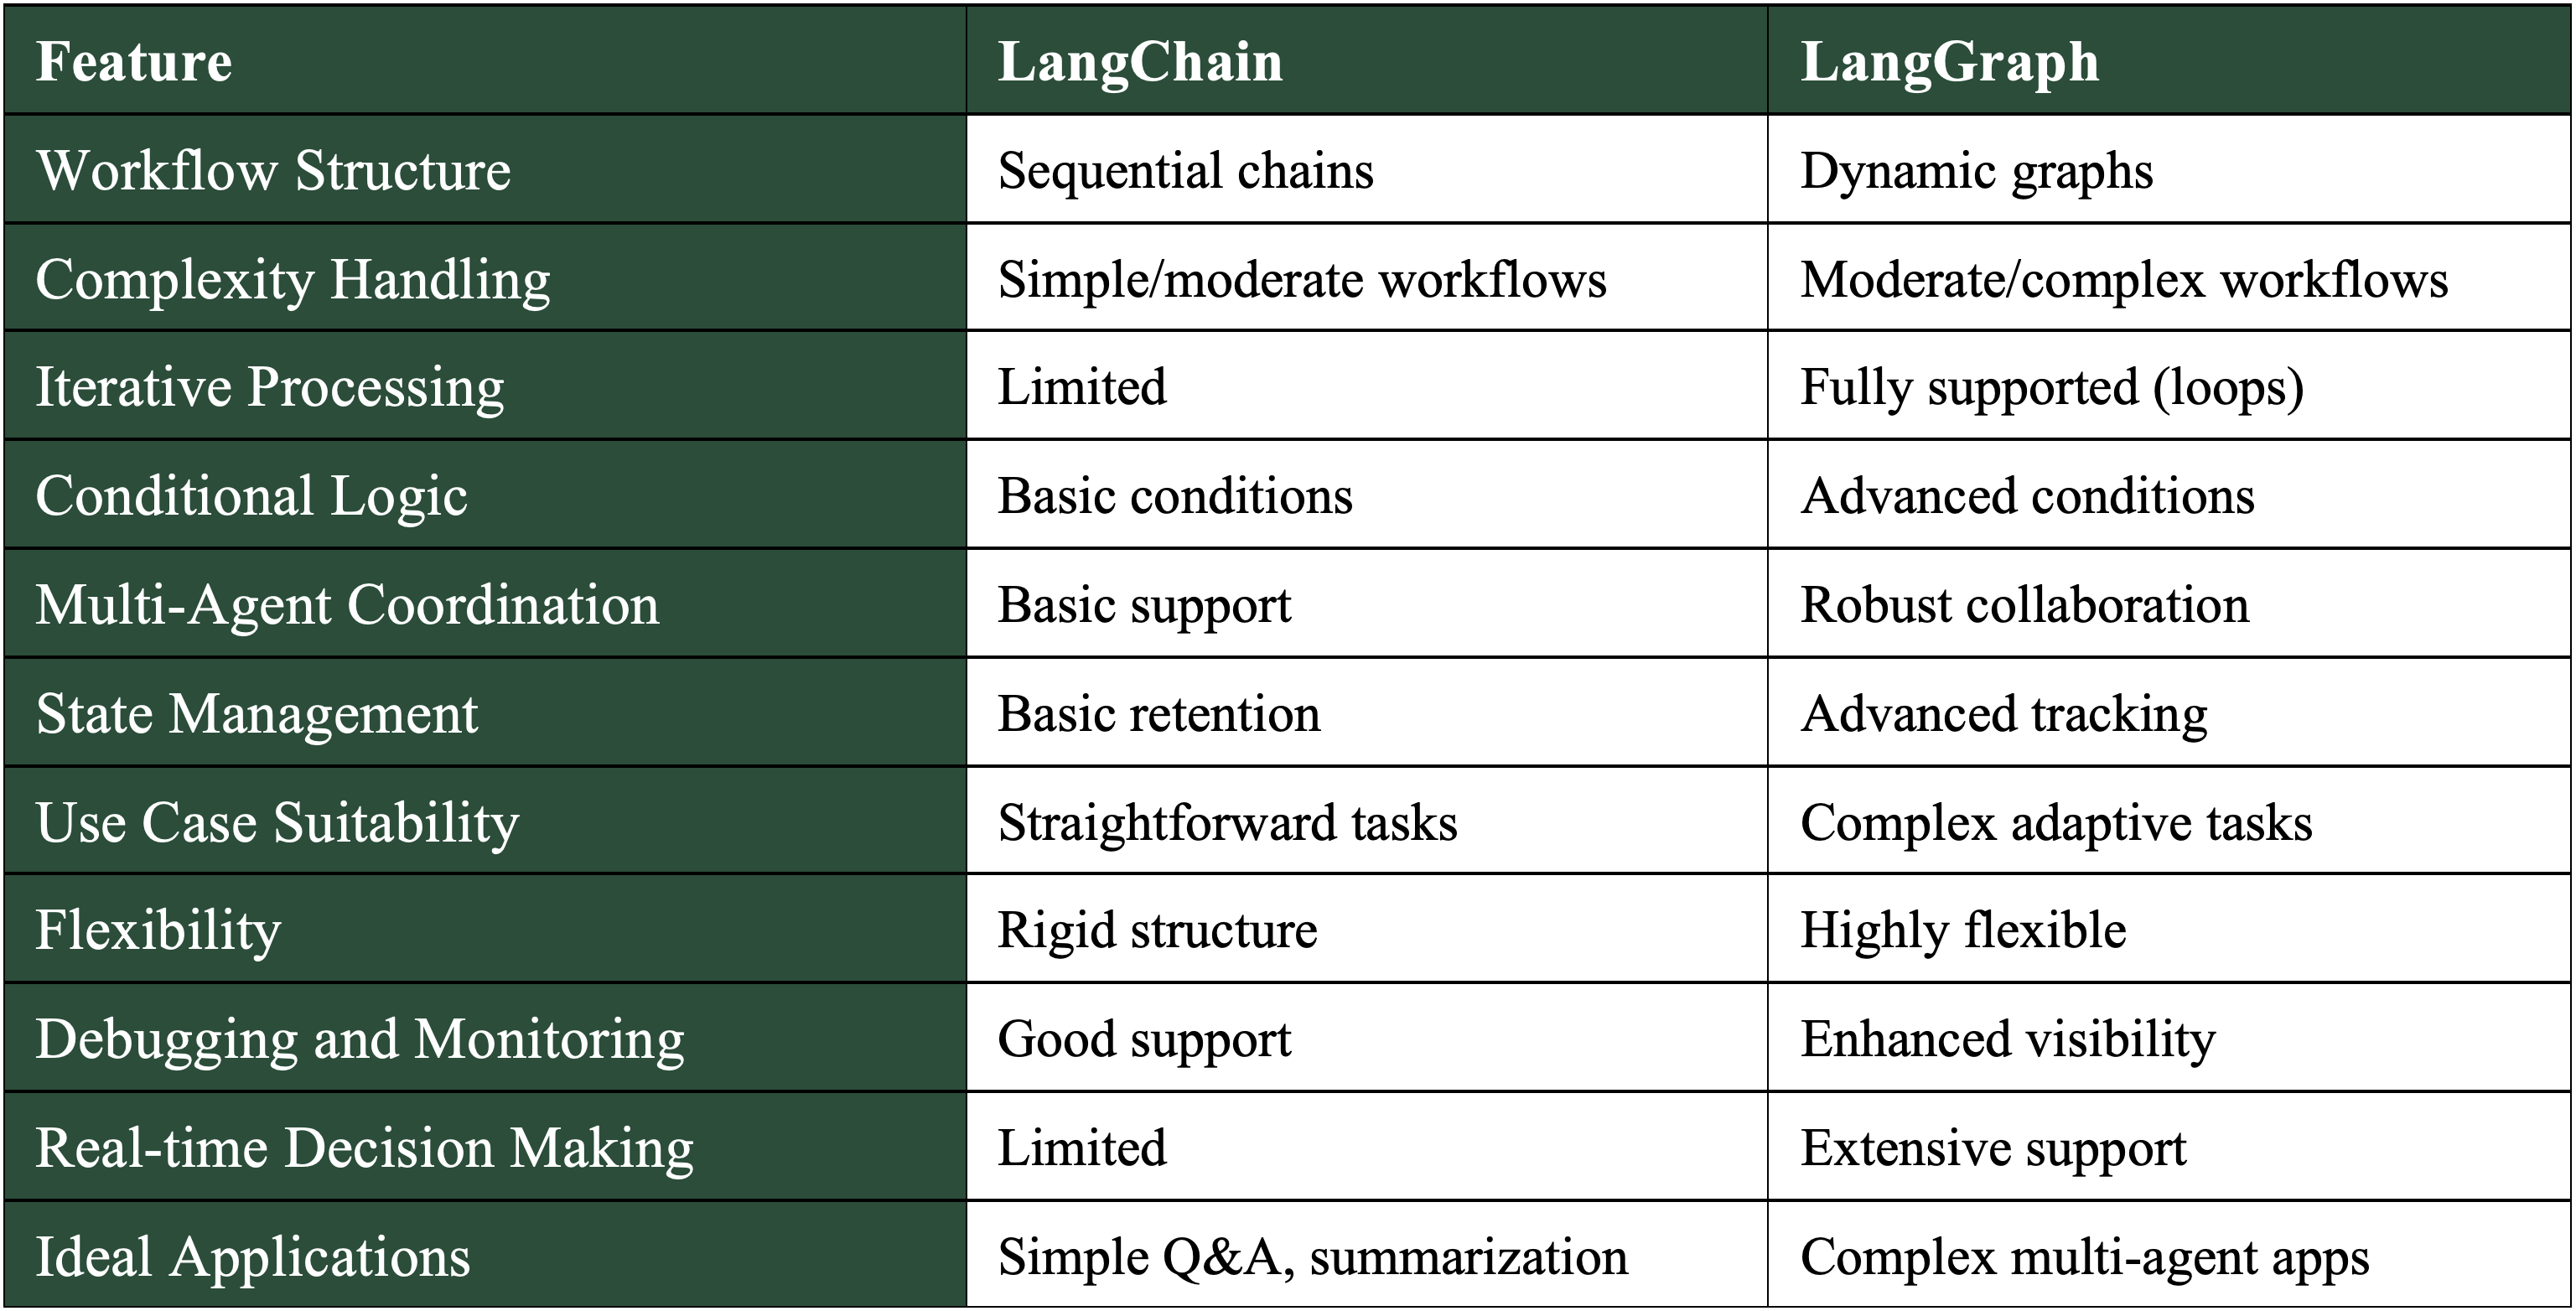
\includegraphics[width=1\textwidth]{Images/Comparison of LangChain and LangGraph.png}
    \captionof{table}{Comparison of LangChain and LangGraph}
    \label{tab:langchain_langgraph_comparison}
\end{center}

The choice between these frameworks thus depends primarily on the complexity of the intended application, where LangChain offers simplicity for linear scenarios, while LangGraph is suited for adaptive, complex applications requiring enhanced flexibility and sophisticated state management.

% Langfuse and Observability
\subsection{Langfuse and Observability}

% Overview
\subsubsection{Overview}
Langfuse is an open-source observability platform designed specifically for applications powered by Large Language Models (LLMs). It provides developers with tools to trace, debug, and analyze the behavior of LLM applications, ensuring better performance and reliability.

\begin{center}
    \centering
    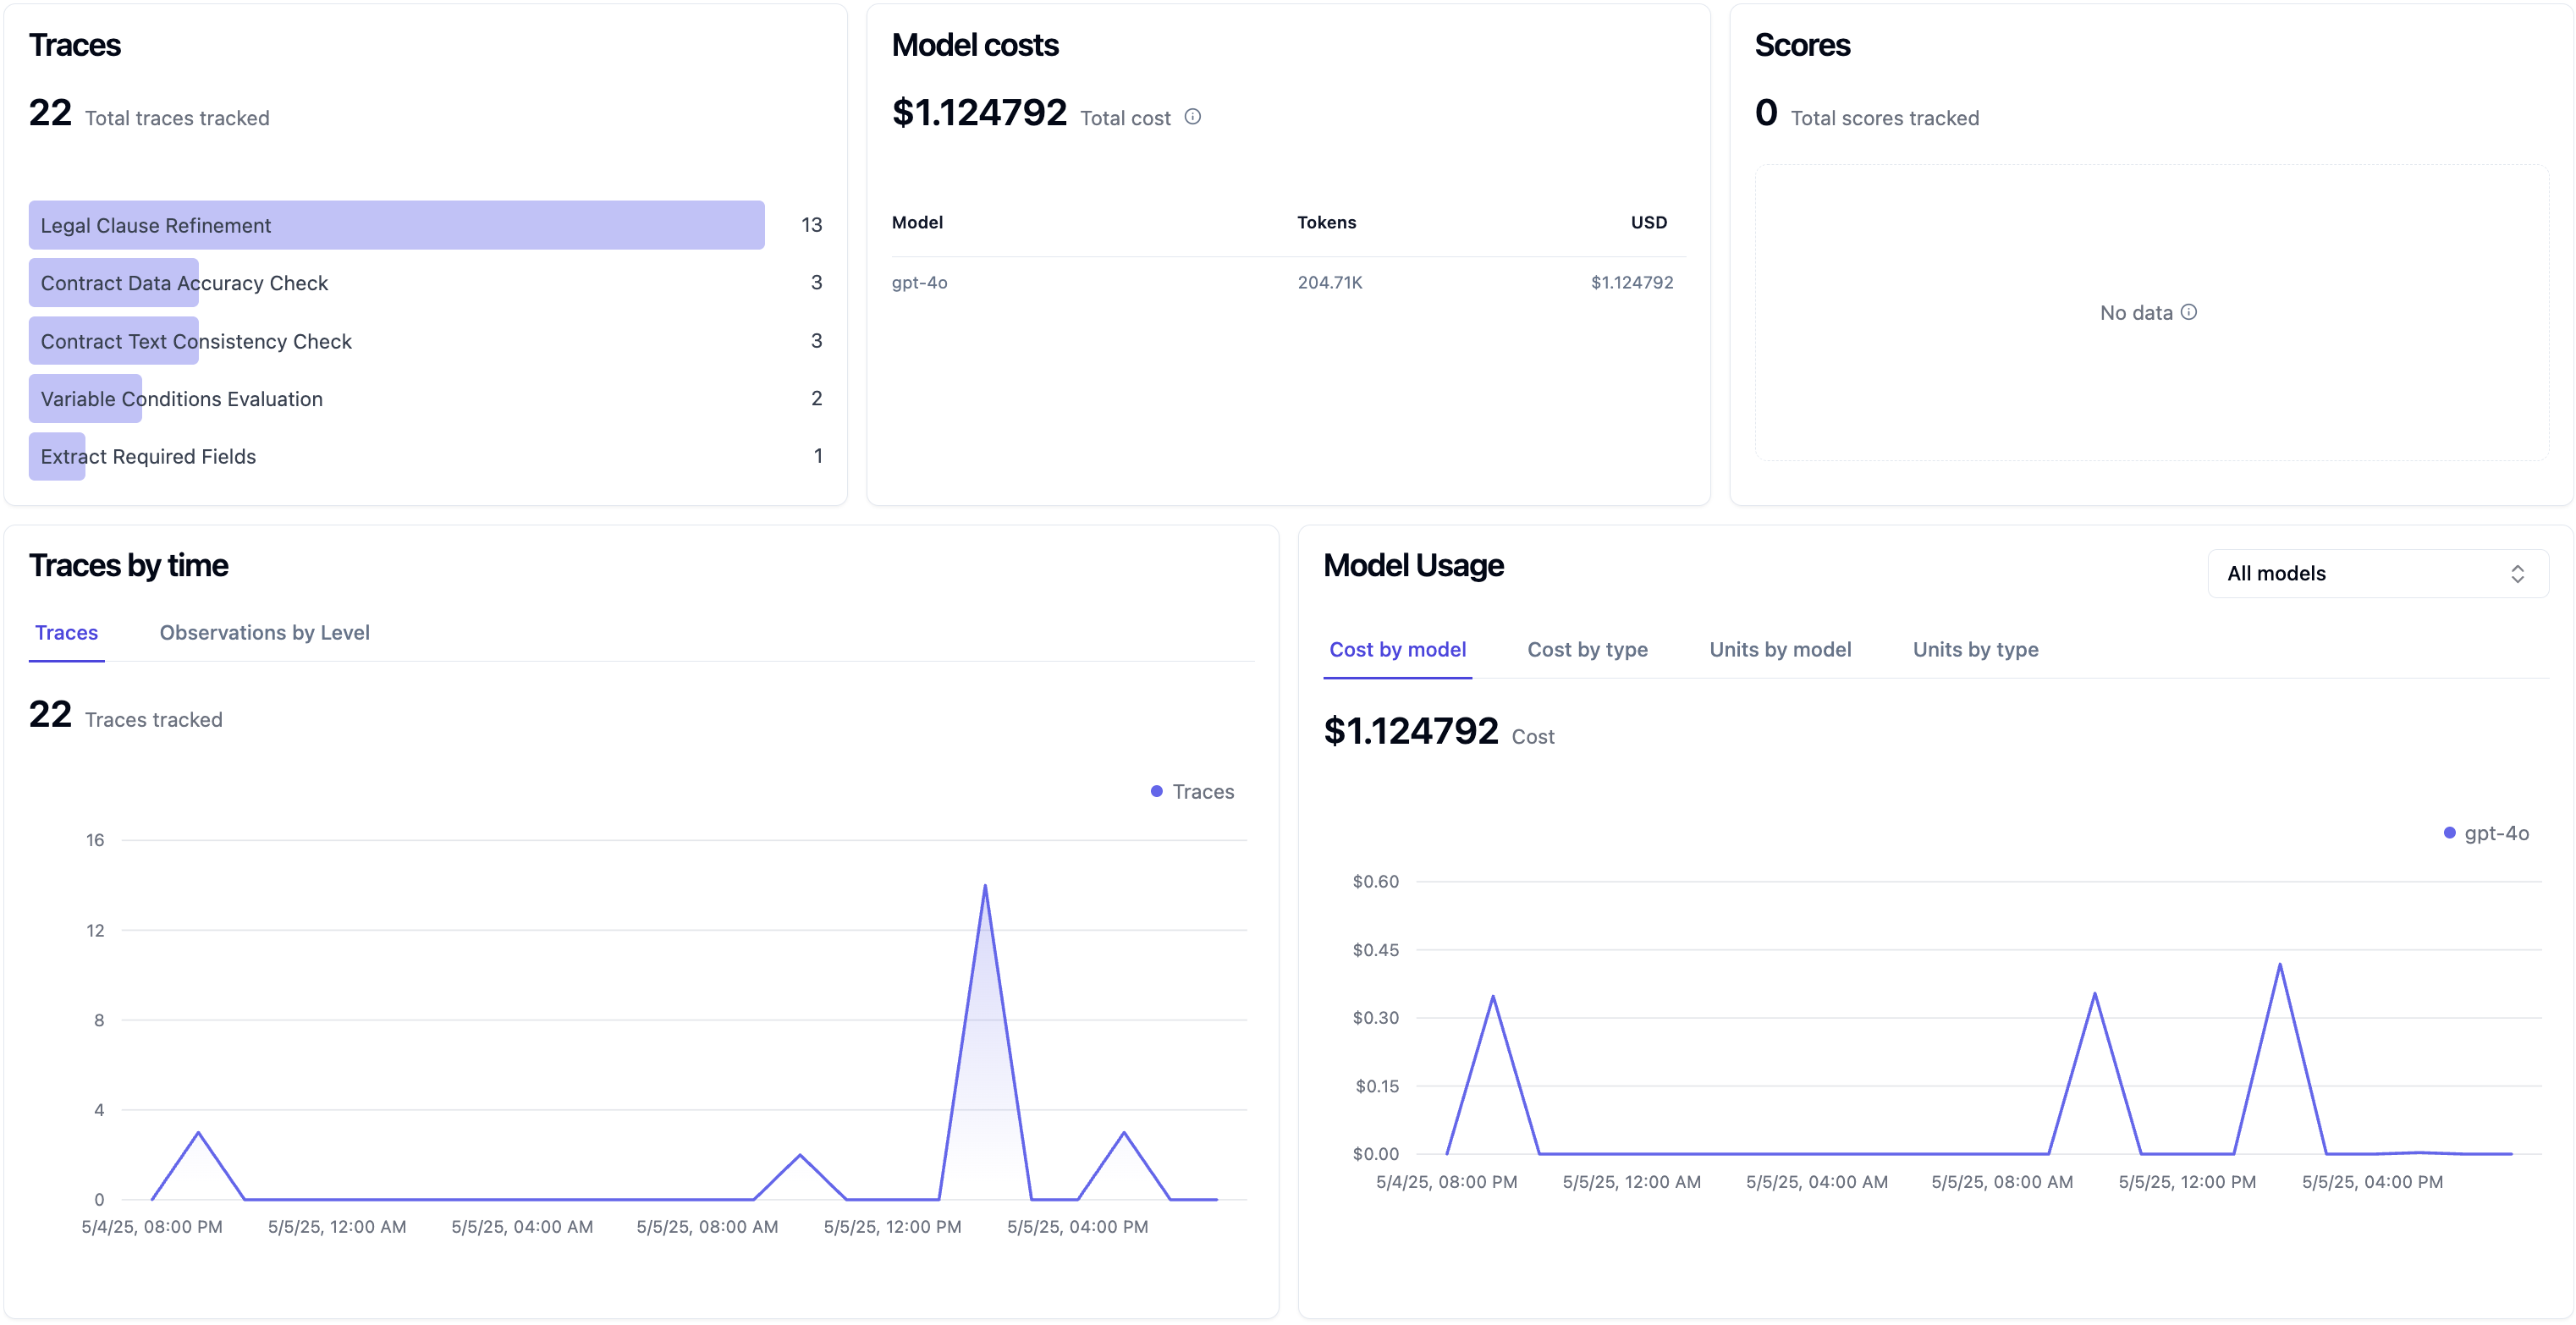
\includegraphics[width=1\textwidth]{Images/Langfuse Overview.png}
    \captionof{figure}{Langfuse Dashboard}
    \label{fig:langfuseDashboard}
\end{center}

% Key Features
\subsubsection{Key Features}
\begin{itemize}
    \item \textbf{Comprehensive Tracing}: Langfuse captures detailed traces of LLM operations, including prompts, responses, and intermediate steps, allowing developers to understand the flow of data and identify issues effectively.
    \item \textbf{Session Management}: It groups related interactions into sessions, providing a holistic view of multi-turn conversations or complex workflows.
    \item \textbf{Analytics Dashboard}: Langfuse offers dashboards that display metrics such as latency, token usage, and cost, enabling teams to monitor and optimize application performance.
    \item \textbf{Prompt Management}: The platform includes tools for managing and versioning prompts, facilitating experimentation and iterative development.
    \item \textbf{Integration Support}: Langfuse integrates seamlessly with popular frameworks like LangChain, LlamaIndex, and OpenAI SDKs, as well as supports OpenTelemetry for broader observability needs.
\end{itemize}

% Deployment Options
\subsubsection{Deployment Options}
Langfuse can be deployed in various environments:

\begin{itemize}
    \item \textbf{Cloud Hosting}: Utilize Langfuse’s managed cloud service for quick setup and scalability.
    \item \textbf{Self-Hosting}: Deploy Langfuse on-premises or in private clouds using Docker, providing full control over data and configurations.
\end{itemize}

% Use Cases
\subsubsection{Use Cases}
\begin{itemize}
    \item \textbf{Debugging Complex Workflows}: By tracing each step of LLM operations, developers can pinpoint and resolve issues in complex applications.
    \item \textbf{Performance Monitoring}: Track metrics to identify bottlenecks and optimize resource usage.
    \item \textbf{Quality Assurance}: Analyze user interactions and feedback to improve response quality and user satisfaction.
    \item \textbf{Compliance and Auditing}: Maintain detailed logs for auditing purposes, ensuring compliance with regulatory standards.
\end{itemize}

Incorporating Langfuse into the development lifecycle of LLM applications enhances transparency, reliability, and efficiency, making it an invaluable tool for teams aiming to build robust AI solutions.

% Tiptap for Rich Text Editing
\subsection{Tiptap for Rich Text Editing}

% Overview
\subsubsection{Overview}
Tiptap is a headless, open-source rich text editor framework built on ProseMirror, designed for developers seeking full control over their content editing interfaces. Its modular architecture and extensive extension ecosystem make it a powerful tool for building customized, collaborative, and AI-enhanced editing experiences.

\begin{center}
    \centering
    
\includegraphics[width=0.8\textwidth]{Images/Tiptap editor.jpg}
    \captionof{figure}{Tiptap Editor} \cite{tiptap_editor}
    \label{fig:tiptap_editor}
\end{center}

% Architecture and Core Concepts
\subsubsection{Architecture and Core Concepts}
Tiptap is a headless, framework-agnostic rich text editor built on top of ProseMirror, designed to provide developers with full control over the editor’s functionality and appearance. Its architecture is modular and extensible, allowing for the creation of customized editing experiences.

\begin{center}
    \centering
    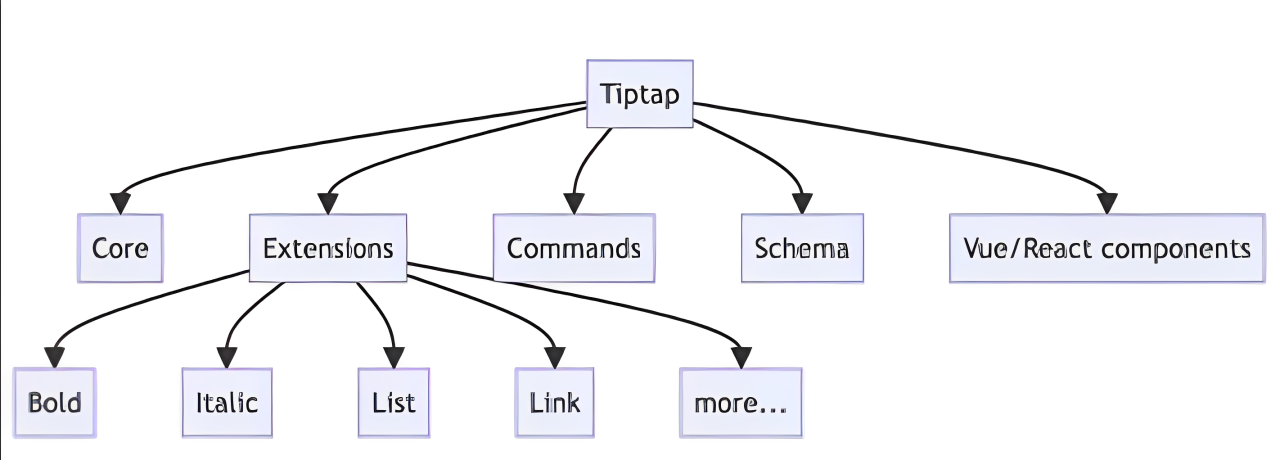
\includegraphics[width=0.8\textwidth]{Images/Tiptap Architecture.png}
    \captionof{figure}{Tiptap Architecture}
    \label{fig:tiptapArchitecture}
\end{center}

Key Architectural Components:
\begin{itemize}
    \item \textbf{Schema}: Defines the structure of the document, specifying the allowed nodes (e.g., paragraphs, headings) and marks (e.g., bold, italic). This strict schema ensures content consistency and predictability.
    \item \textbf{State}: Represents the current content and selection within the editor. It is immutable and updated through transactions, enabling features like undo/redo and collaborative editing.
    \item \textbf{Transaction}: Encapsulates changes to the state, such as text insertions or formatting. Transactions ensure that state changes are predictable and manageable.
    \item \textbf{Extensions}: Modular units that add functionality to the editor, such as new nodes, marks, commands, or plugins. Tiptap provides a rich set of core and community extensions, and developers can create custom ones as needed.
    \item \textbf{Commands}: Functions that perform actions within the editor, often used to manipulate the document or respond to user input. Commands can be chained for complex operations.
\end{itemize}

% Key Features
\subsubsection{Key Features}
\begin{itemize}
    \item \textbf{Extension-Based Modularity}: Tiptap offers over 100 extensions, including both open-source and Pro options, allowing developers to tailor the editor’s functionality to specific needs.
    \item \textbf{Real-Time Collaboration}: Through integrations like Hocuspocus and CRDTs, Tiptap supports collaborative editing with features like live cursors and offline synchronization.
    \item \textbf{AI Integration}: The Content AI extension enables in-editor AI capabilities such as text suggestions, translations, and content generation, enhancing the writing experience.
    \item \textbf{Framework Agnostic}: Tiptap’s design allows it to be integrated into various JavaScript frameworks, providing flexibility in application development.
\end{itemize}

% Use Cases
\subsubsection{Use Cases}
Tiptap is suitable for a wide range of applications, including:
\begin{itemize}
    \item Building Notion-like editors with custom blocks and interactions.
    \item Developing collaborative document editing platforms.
    \item Creating AI-assisted writing tools with real-time suggestions.
    \item Implementing rich text editors in CMS platforms. 
\end{itemize}    

Tiptap stands out as a versatile and developer-friendly rich text editor framework. Its combination of headless architecture, modular extensions, and support for real-time collaboration and AI integration makes it a compelling choice for modern web applications requiring customized content editing solutions.

% Project Requirements
\section{Specification of Requirements}
Given the agile nature of the project, the actors as well as functional and non-functional requirements are subject to evolve. The elements below reflect the current state of the project.

% Business Architecture
\subsection{Business Architecture}
The business architecture depicted in Figure~\ref{fig:business_architecture} outlines the overarching structure and planned components of the intelligent contract management platform. The platform integrates three main components supported by robust underlying layers of data management, security, observability, and tool integration capabilities.

\begin{center}
    \centering
    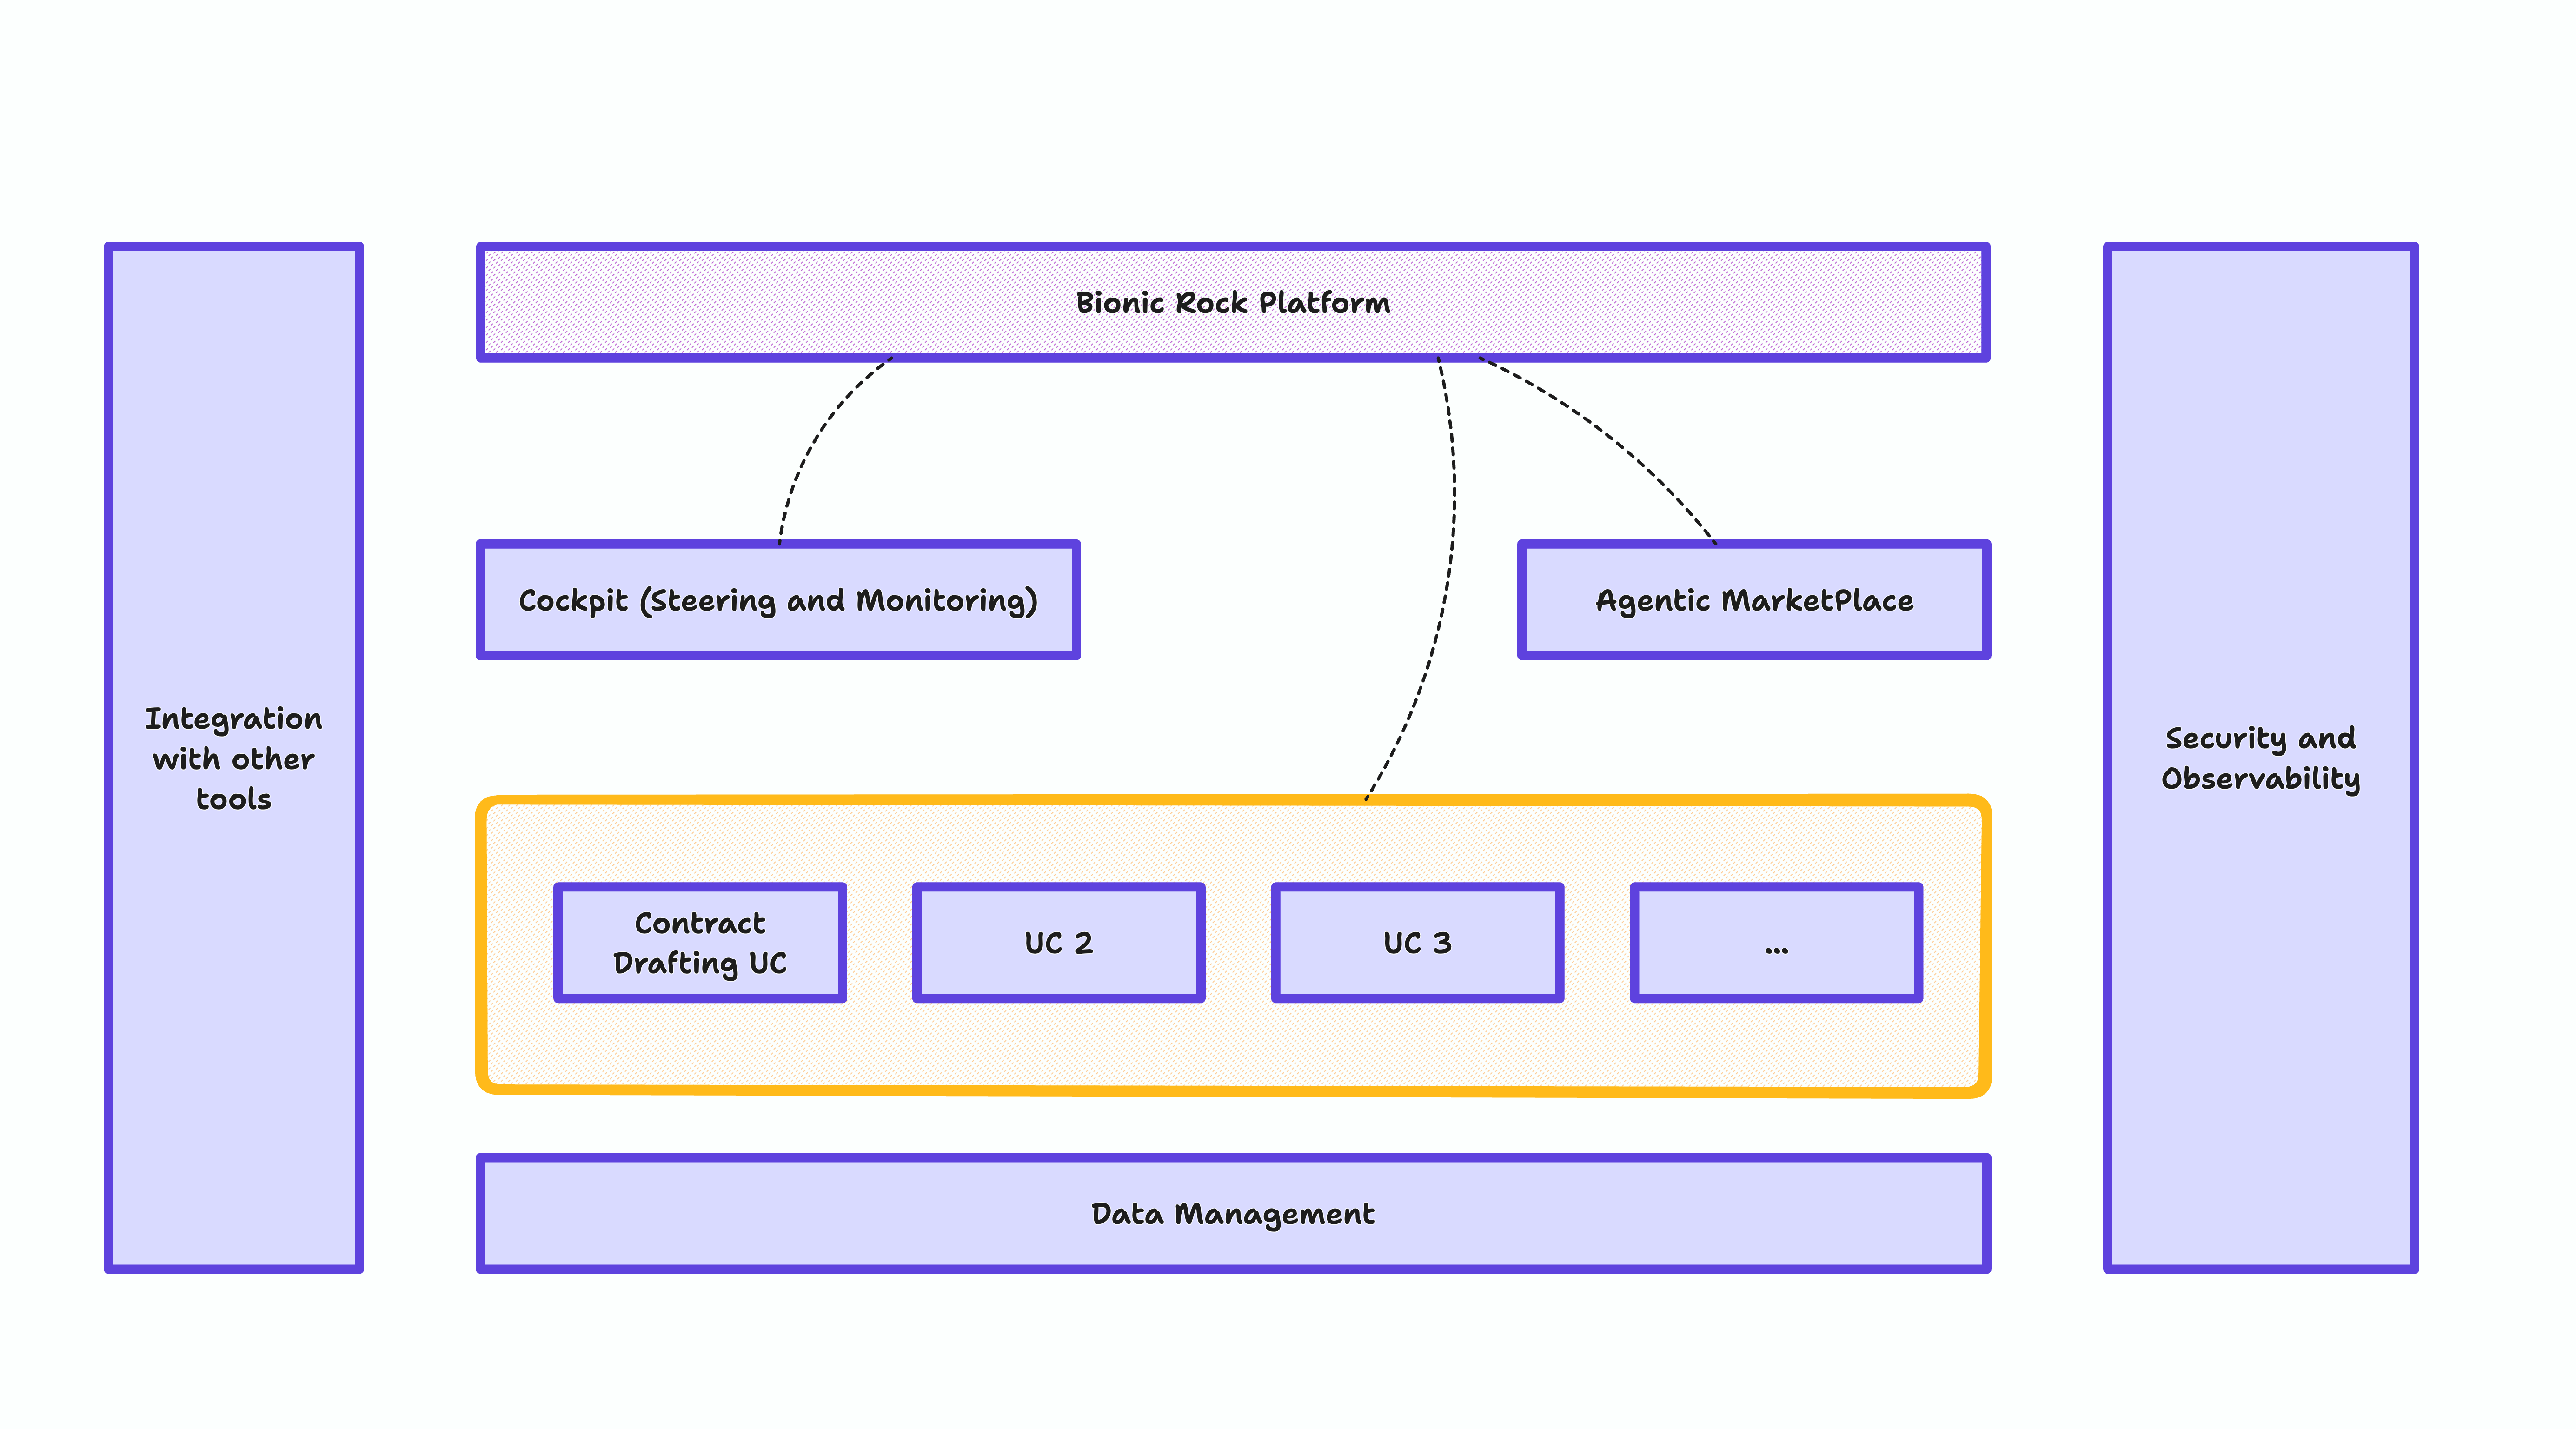
\includegraphics[width=0.9\textwidth]{Images/Business Architecture.png}
    \captionof{figure}{Business Architecture Overview}
    \label{fig:business_architecture}
\end{center}

The platform structure is organized into three core areas:

\begin{itemize}
\item \textbf{Cockpit (Steering and Monitoring)}: This area provides oversight and real-time analytics, enabling stakeholders to monitor system performance, track usage, and manage workflows effectively.
\item \textbf{Agentic Marketplace}: Designed to host various autonomous AI agents, this component facilitates the scalable deployment and orchestration of intelligent services, supporting diverse, dynamic business needs and agent interactions.
\item \textbf{Use Case Features}: These represent modular functionalities tailored to specific business processes. The primary use case currently prioritized is the \textbf{Contract Drafting Use Case (UC)}, scheduled for completion within a 21-week timeframe. This use case is central to my internship project and focuses on automating and enhancing the contract drafting process through intelligent clause selection, AI-assisted drafting, compliance verification, and collaboration enhancements.
\end{itemize}

These foundational components are encapsulated within a broader environment of:

\begin{itemize}
\item \textbf{Data Management}: Ensures consistent data governance, quality, and efficient access to support the platform's intelligent features.
\item \textbf{Integration with Other Tools}: Provides seamless interoperability with external and internal enterprise applications, extending the platform's capabilities and ensuring a cohesive user experience.
\item \textbf{Security and Observability}: Delivers comprehensive security measures and observability tools to protect data integrity, ensure compliance, and provide transparent system monitoring and diagnostics.
\end{itemize}

This structured business architecture aims to offer a scalable, secure, and integrative platform capable of addressing complex legal operations through advanced technological solutions.

% Actor Identification
\subsection{Actor Identification}
An actor specifies a role played by a user or any other system interacting with the solution. Actors are always external to the system, interacting by initiating a use case, providing inputs, or receiving outputs. In the context of our platform, we have two types of actors:

\begin{center}
    \centering
    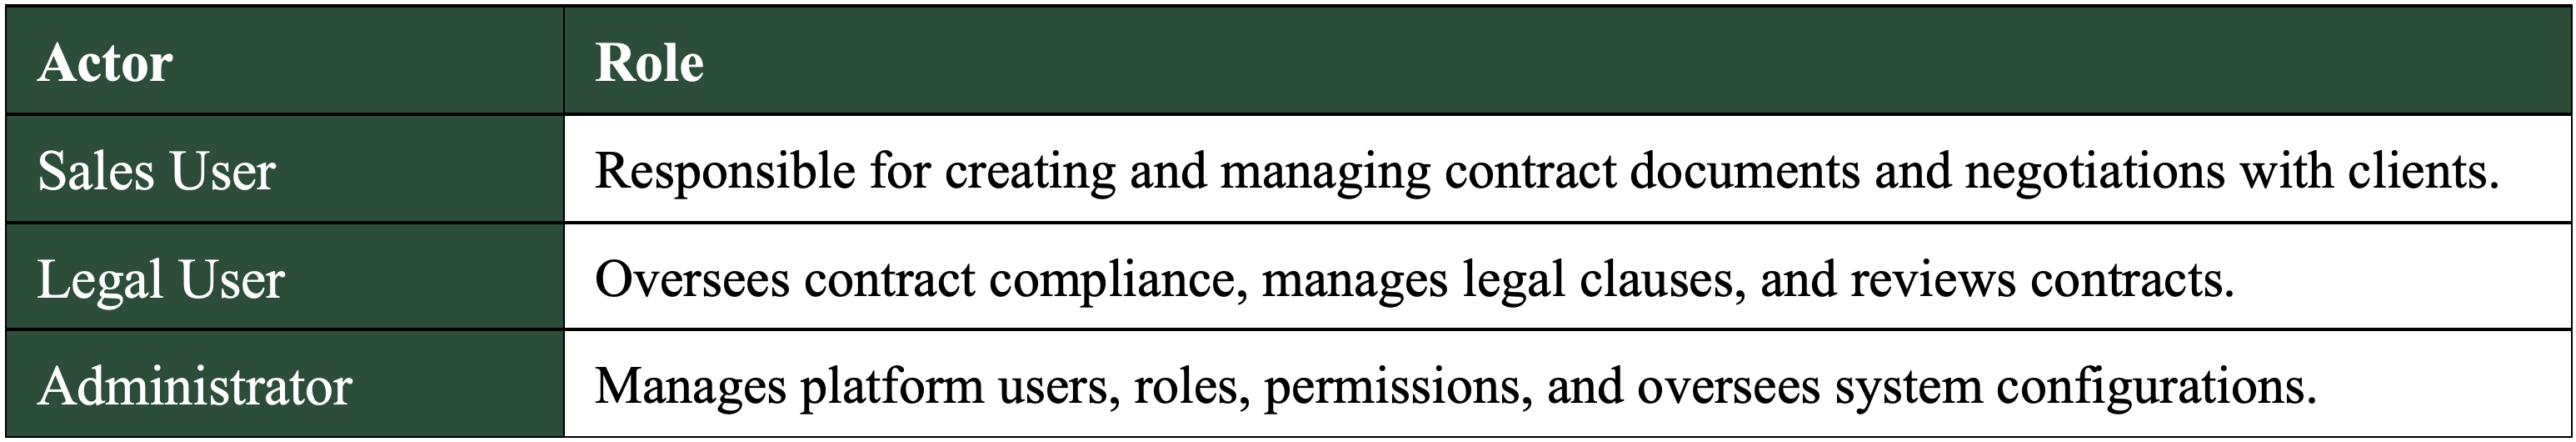
\includegraphics[width=1\textwidth]{Images/Actors and Their Roles.png}
    \captionof{table}{Actors and Their Roles}
    \label{tab:actors_and_roles}
\end{center}

% Functional Requirements
\subsection{Functional Requirements}

% Authentication
\subsubsection{Authentication}
The application must enable users to authenticate using a username or email and password.

% Sales User Functionalities
\subsubsection{Sales User Functionalities}

\textbf{Contract Generation}:\vspace{0.4em}
\begin{adjustwidth}{3em}{1em}
    \begin{itemize}
        \item The sales user must be able to create a new contract.\vspace{0.4em}
        \item The sales user must be able to create a new client.
    \end{itemize}
\end{adjustwidth}\vspace{0.85em}

\textbf{Contract Editing}:\vspace{0.4em}
\begin{adjustwidth}{3em}{1em}
    \begin{itemize}
        \item The Sales user must be able to access the rich-text contract editor.\vspace{0.4em}
        \item The Sales user must be able to create clause requests.\vspace{0.4em}
        \item The Sales user must be able to modify contract variables.\vspace{0.4em}
        \item The Sales user must be able to track changes across different contract versions.  
    \end{itemize}
\end{adjustwidth}\vspace{0.85em} 

\textbf{Contract Review \& Compliance}:\vspace{0.4em}
\begin{adjustwidth}{3em}{1em}
    \begin{itemize}
        \item The Sales user must be able to trigger AI-powered compliance checks.\vspace{0.4em}
        \item The Sales user must be able to change the contract status (e.g., in editing, in review, finalized).
    \end{itemize}
\end{adjustwidth}\vspace{0.85em} 

\textbf{Export, Sharing, and Management}:\vspace{0.4em}
\begin{adjustwidth}{3em}{1em}
    \begin{itemize}
        \item The Sales user must be able to access only the contracts they have created.\vspace{0.4em}
        \item The Sales user must be able to export contracts as downloadable files (Word, PDF).\vspace{0.4em}
        \item The Sales user must be able to share contracts via secure links or email attachments.\vspace{0.4em}
        \item The Sales user must be able to archive and delete contracts.
    \end{itemize}
\end{adjustwidth}\vspace{0.85em}  

% Legal User Functionalities
\subsubsection{Legal User Functionalities}

\textbf{Clause Management}:\vspace{0.4em}
\begin{adjustwidth}{3em}{1em}
    \begin{itemize}
        \item The Legal user must be able to review clause requests from Sales.\vspace{0.4em}
        \item The Legal user must be able to refine clause content using AI assistance.\vspace{0.4em}
        \item The Legal user must be able to create, insert, modify, and delete legal clauses.  
    \end{itemize}
\end{adjustwidth}\vspace{0.85em} 

\textbf{Contract Editing and Versioning}:\vspace{0.4em}
\begin{adjustwidth}{3em}{1em}
    \begin{itemize}
        \item The Legal user must be able to access and create versions of contracts.\vspace{0.4em}
        \item The Legal user must be able to restore previous contract versions.\vspace{0.4em}
        \item The Legal user must be able to edit contracts using a rich-text editor.\vspace{0.4em}
        \item The Legal user must be able to modify contract variables.
    \end{itemize}
\end{adjustwidth}\vspace{0.85em} 

\textbf{Contract Review \& Compliance}:\vspace{0.4em}
\begin{adjustwidth}{3em}{1em}
    \begin{itemize}
        \item The Legal user must be able to trigger AI-powered compliance checks.\vspace{0.4em}
        \item The Legal user must be able to change the status of a contract (e.g., in editing, in review).
    \end{itemize}
\end{adjustwidth}\vspace{0.85em} 

\textbf{Export, Sharing, and Management}:\vspace{0.4em}
\begin{adjustwidth}{3em}{1em}
    \begin{itemize}
        \item The Legal user must be able to access all existing contracts.\vspace{0.4em}
        \item The Legal user must be able to export contracts as downloadable files (Word, PDF).\vspace{0.4em}
        \item The Legal user must be able to share contracts via secure links or email attachments.
    \end{itemize}
\end{adjustwidth}\vspace{0.85em} 

% Administrator Functionalities
\subsubsection{Administrator Functionalities}

\textbf{User Management}:\vspace{0.4em}
\begin{adjustwidth}{3em}{1em}
    \begin{itemize}
        \item The administrator must be able to add, modify, or remove platform users.\vspace{0.4em}
        \item The administrator must be able to manage role-based access permissions.
    \end{itemize}
\end{adjustwidth}\vspace{0.85em} 

\textbf{System Configuration}:\vspace{0.4em}
\begin{adjustwidth}{3em}{1em}
    \begin{itemize}
        \item The administrator must be able to configure integration settings and security parameters.\vspace{0.4em}
        \item The administrator must be able to monitor system performance through administrative dashboards.
    \end{itemize}
\end{adjustwidth}\vspace{0.85em} 

% Non-Functional Requirements
\subsection{Non-Functional Requirements}
\begin{itemize}
    \item \textbf{Usability}: High intuitiveness and ease of use for Sales, Legal, and Admin users, promoting efficient adoption across roles.
    \item \textbf{Maintainability}: Modular and well-documented architecture to facilitate smooth updates, debugging, and feature evolution.
    \item \textbf{Security}: Robust access control, secure data handling, and full compliance with applicable legal and organizational standards.
    \item \textbf{System Responsiveness}: Fast UI response, low-latency AI processing, and efficient data retrieval for optimal user experience.
    \item \textbf{Scalability}: Capacity to handle increased user load and data volume while maintaining system performance.
\end{itemize}

% Use Case Diagram
\subsection{Use Case Diagram}
The Use Case Diagram presented in Figure~\ref{fig:use_case_diagram} visually represents the interactions between the identified actors—Sales Users, Legal Users, and Administrators—and the main functionalities offered by the intelligent contract management platform. It illustrates how each user group engages with distinct and shared system features, clearly depicting the overall workflow from contract drafting and editing to compliance verification, version control, and collaboration activities.

\begin{center}
    \centering
    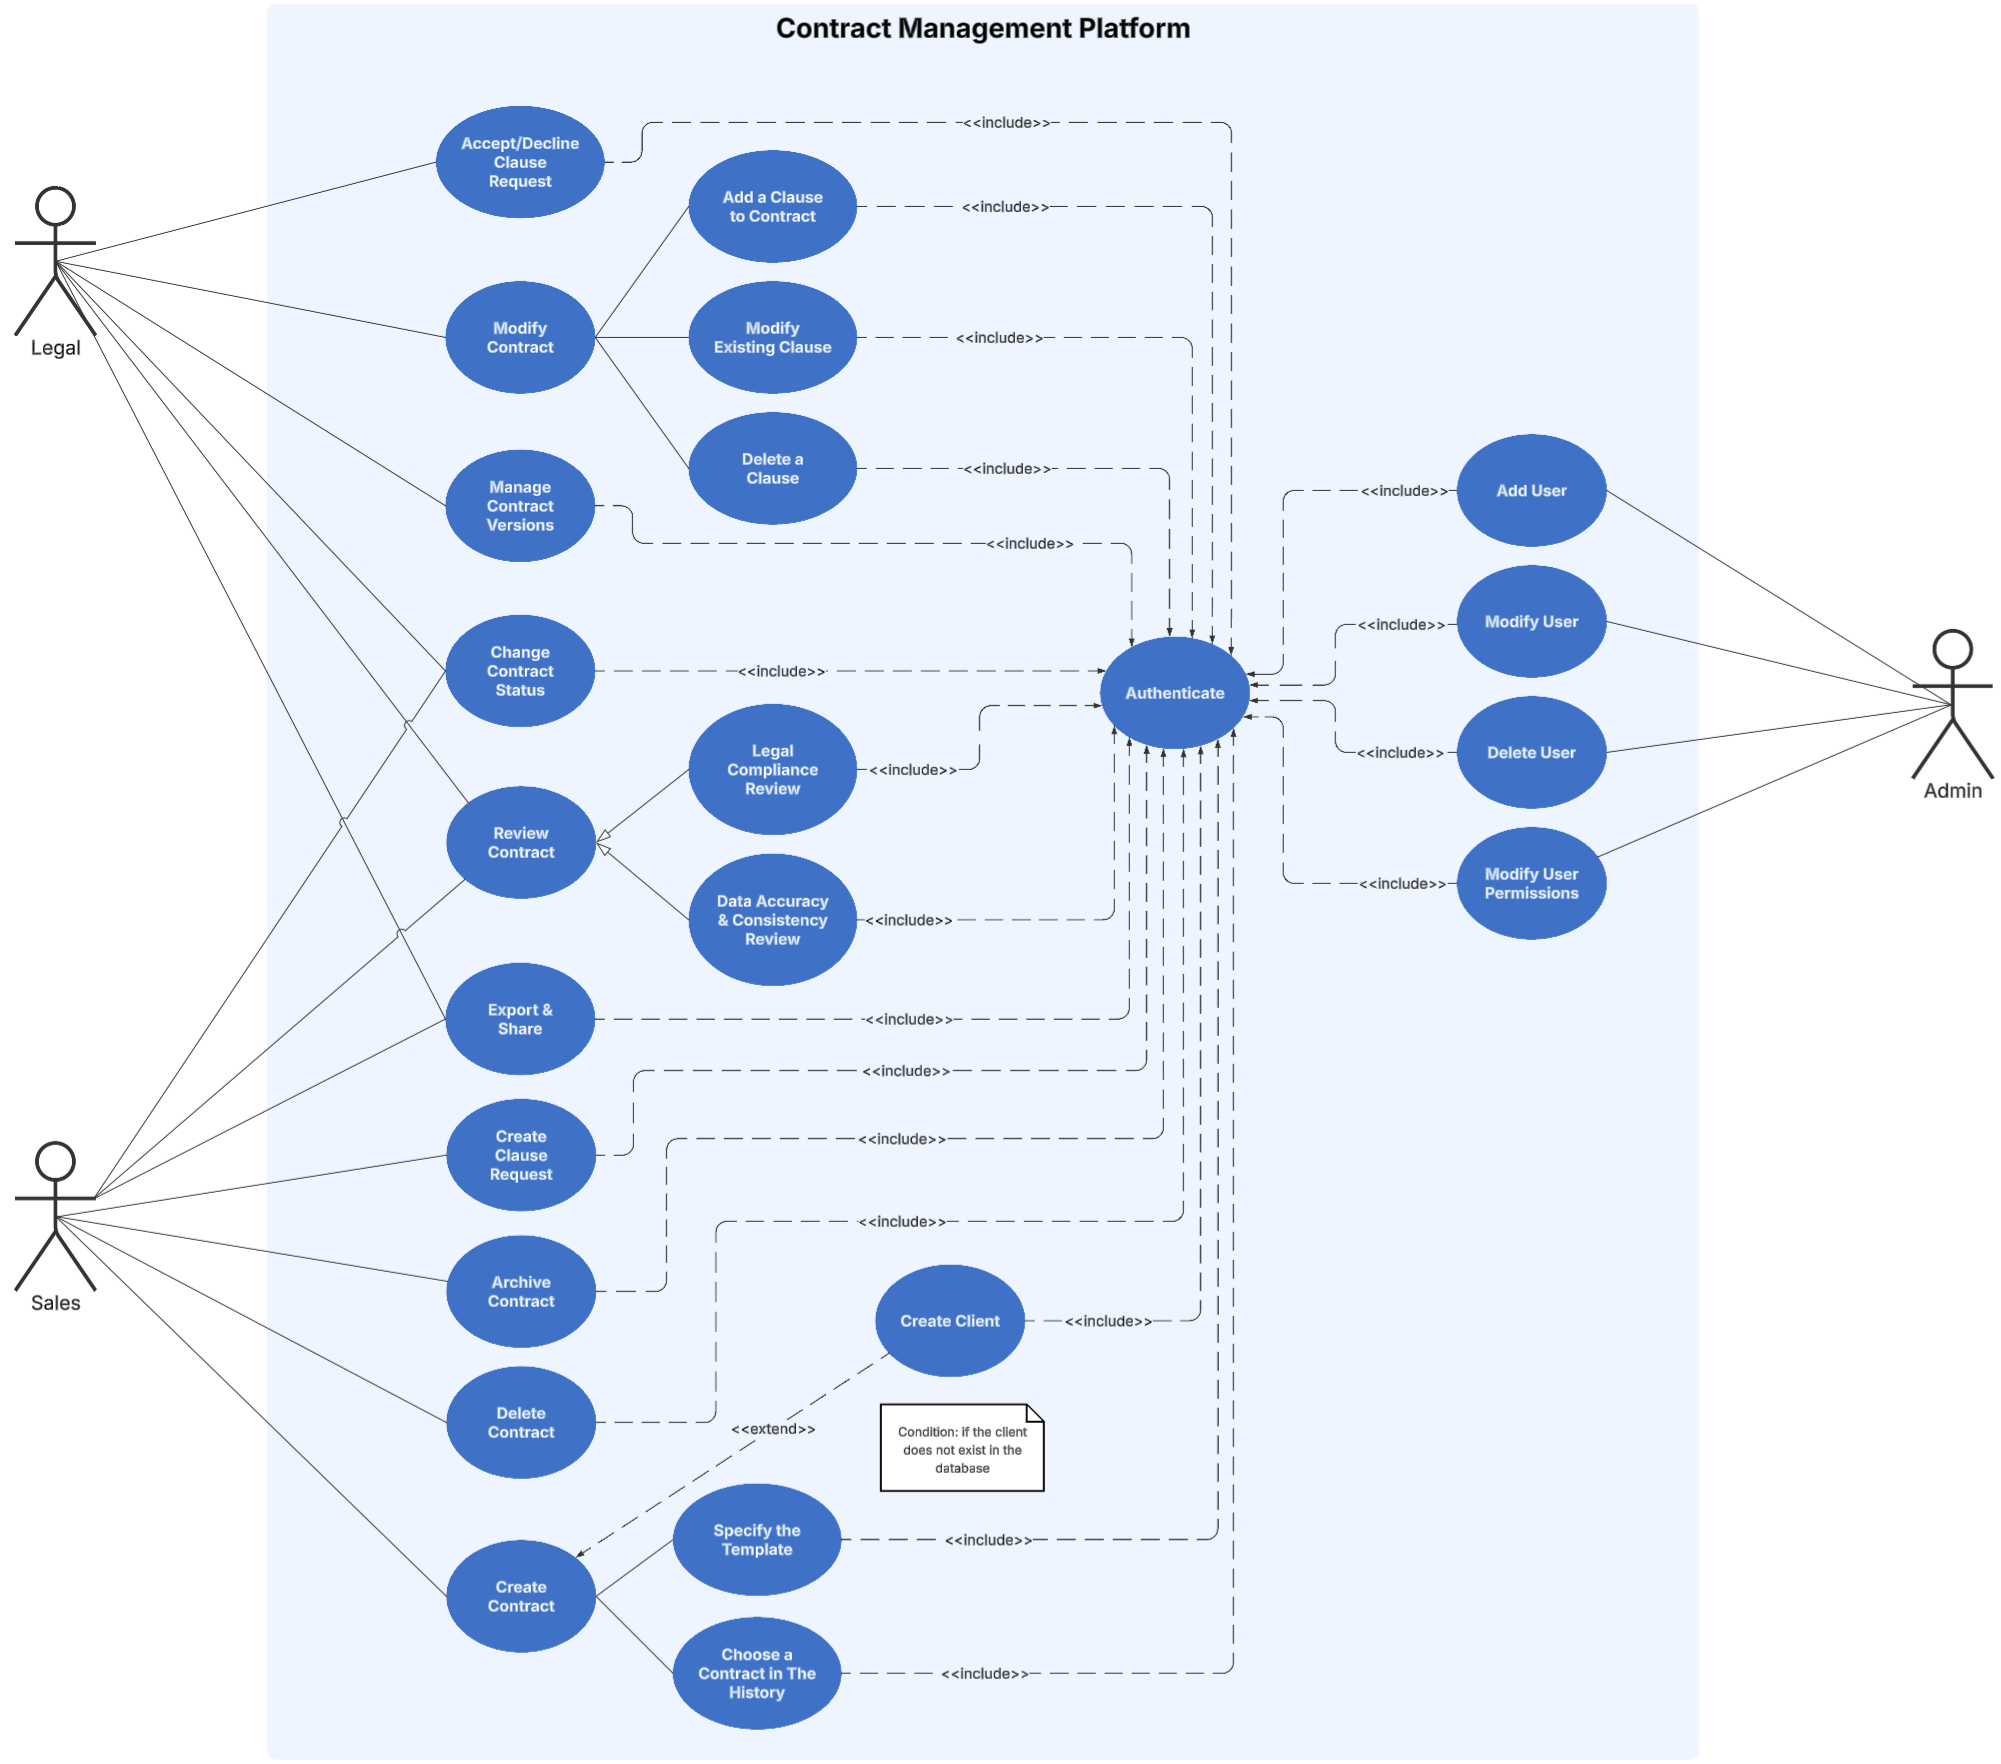
\includegraphics[width=1\textwidth]{Images/Use Case Diagram.png}
    \captionof{figure}{Use Case Diagram}
    \label{fig:use_case_diagram}
\end{center}

% Textual Description
\subsection{Textual Description}

To describe the dynamics of a use case, it is essential to enumerate all interactions between the actor and the system in textual form. This description is crucial, as it facilitates clear communication with all stakeholders and ensures a shared understanding of the business terminology involved.

\textbf{Textual Description of Use Case: Create Contract}\vspace{-0.3cm}

\begin{center}
    \centering
    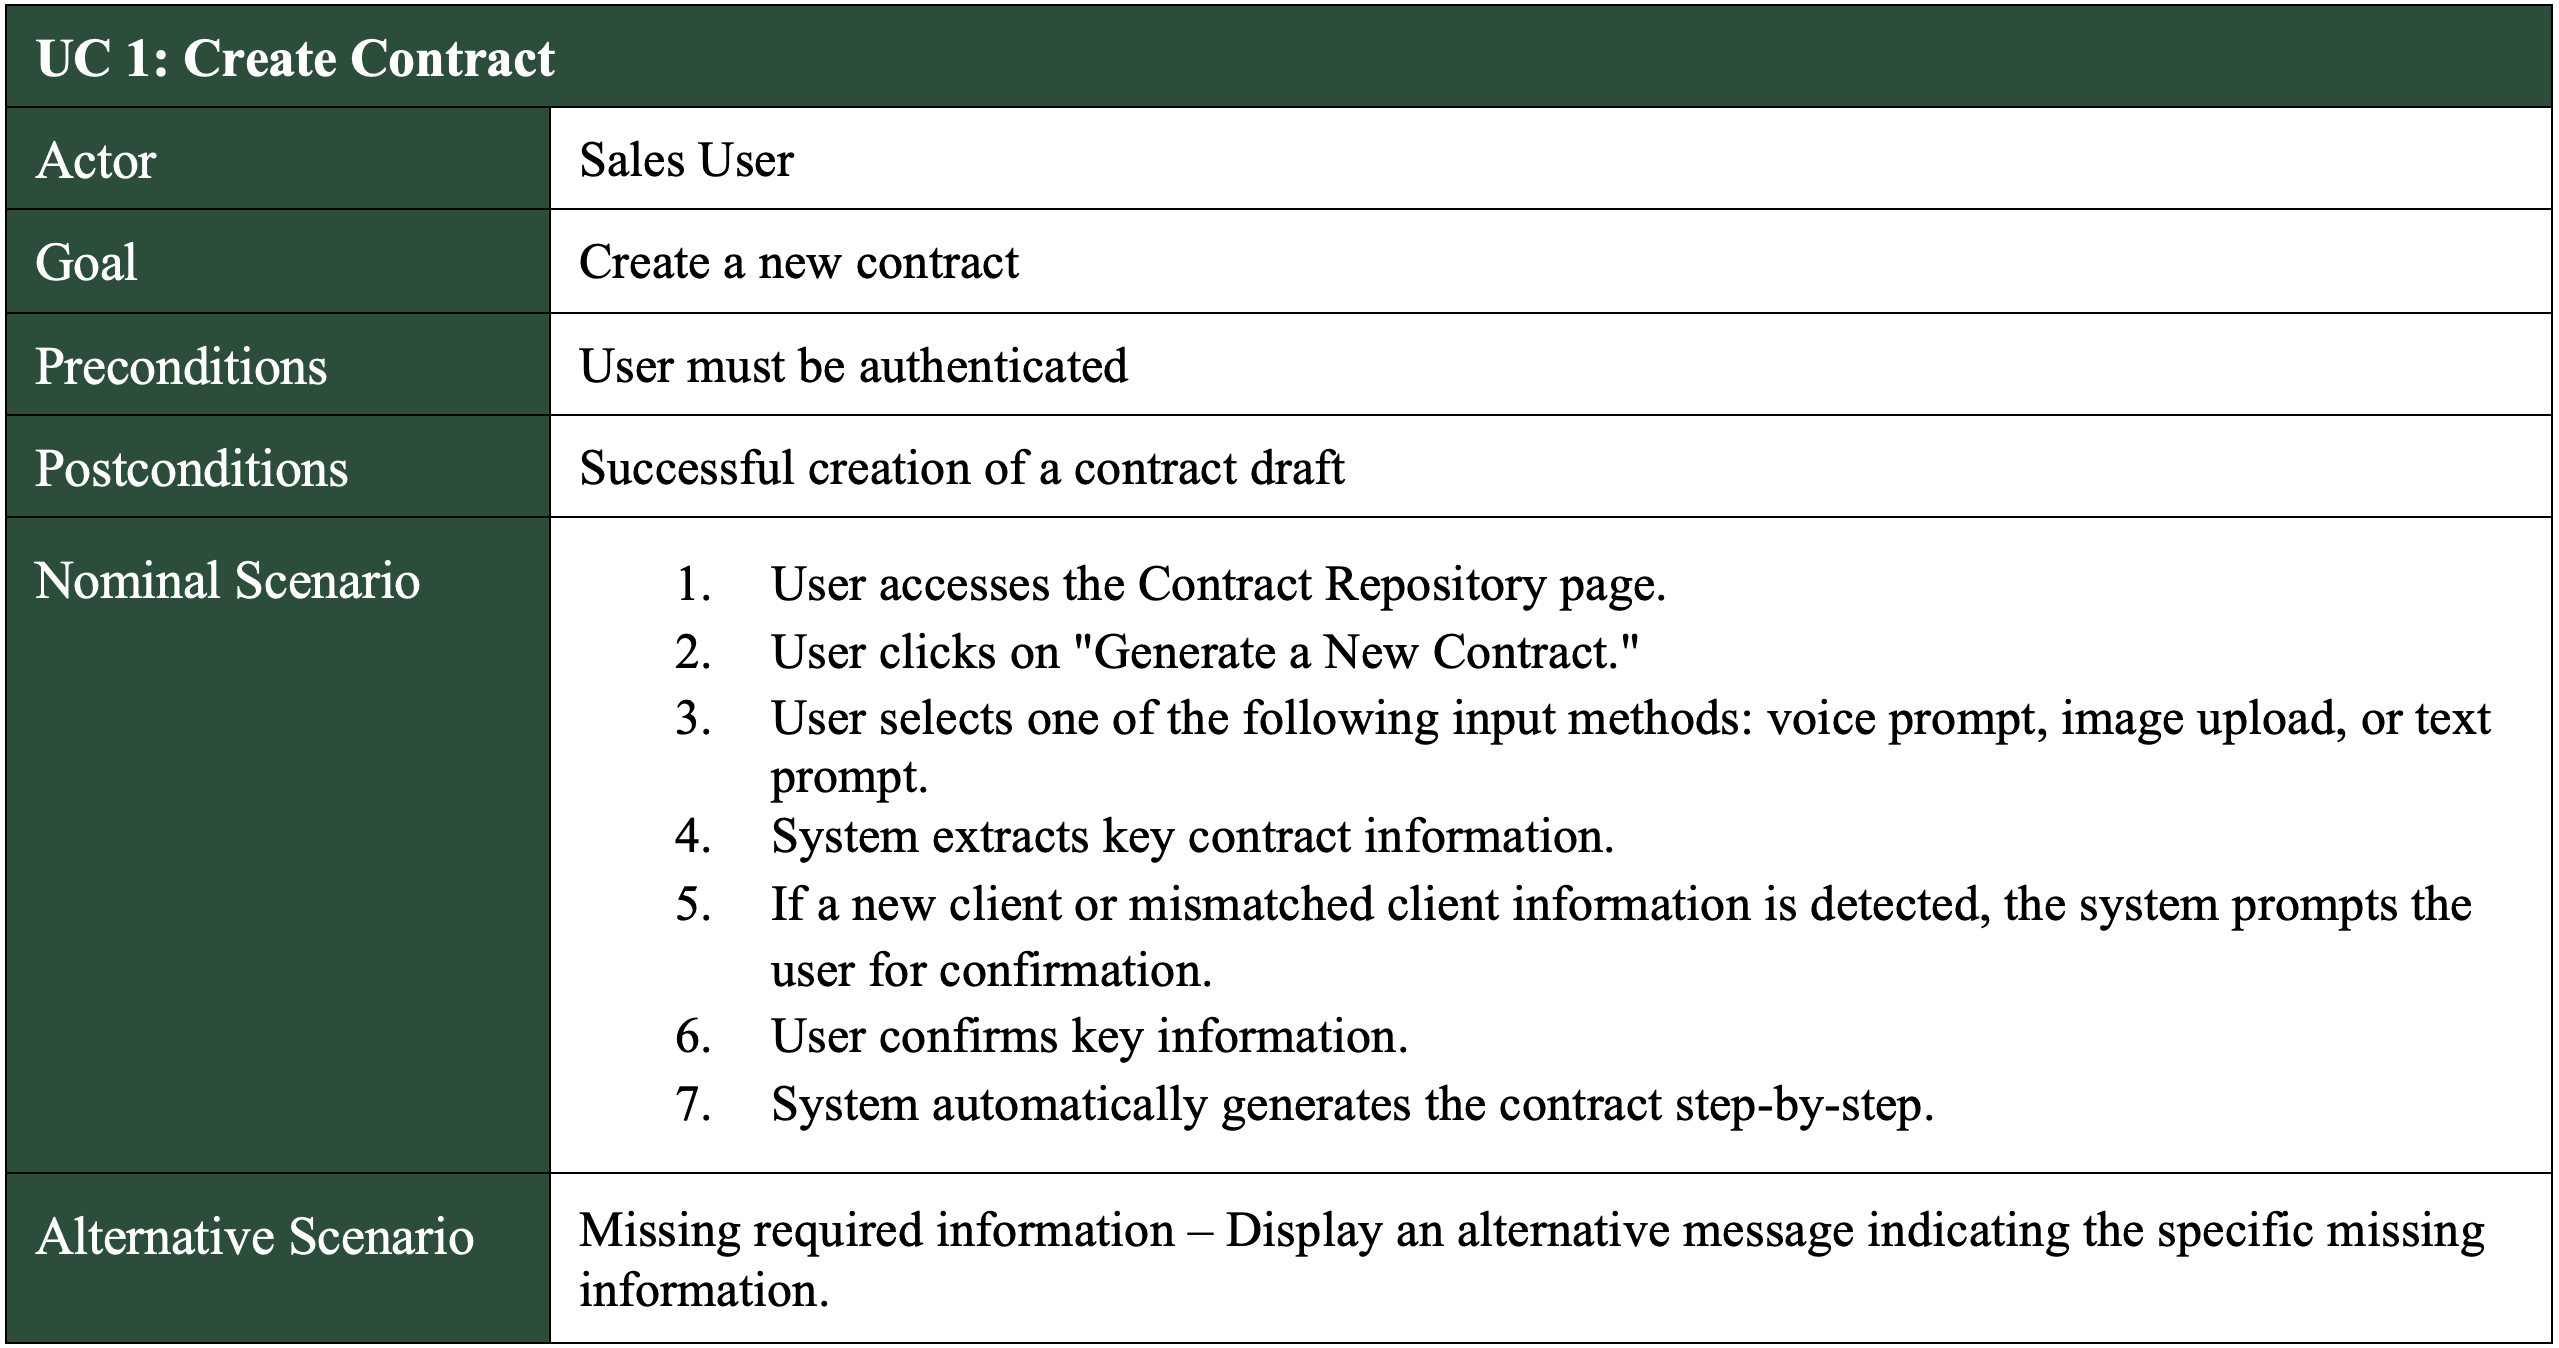
\includegraphics[width=1\textwidth]{Images/Create Contract Use Case.png}
    \captionof{table}{Textual Description of Use Case: Create Contract}
    \label{tab:create_contract_use_case}
\end{center}

\vspace{0.3cm}

\textbf{Textual Description of Use Case: Create Clause Request}\vspace{-0.3cm}

\begin{center}
    \centering
    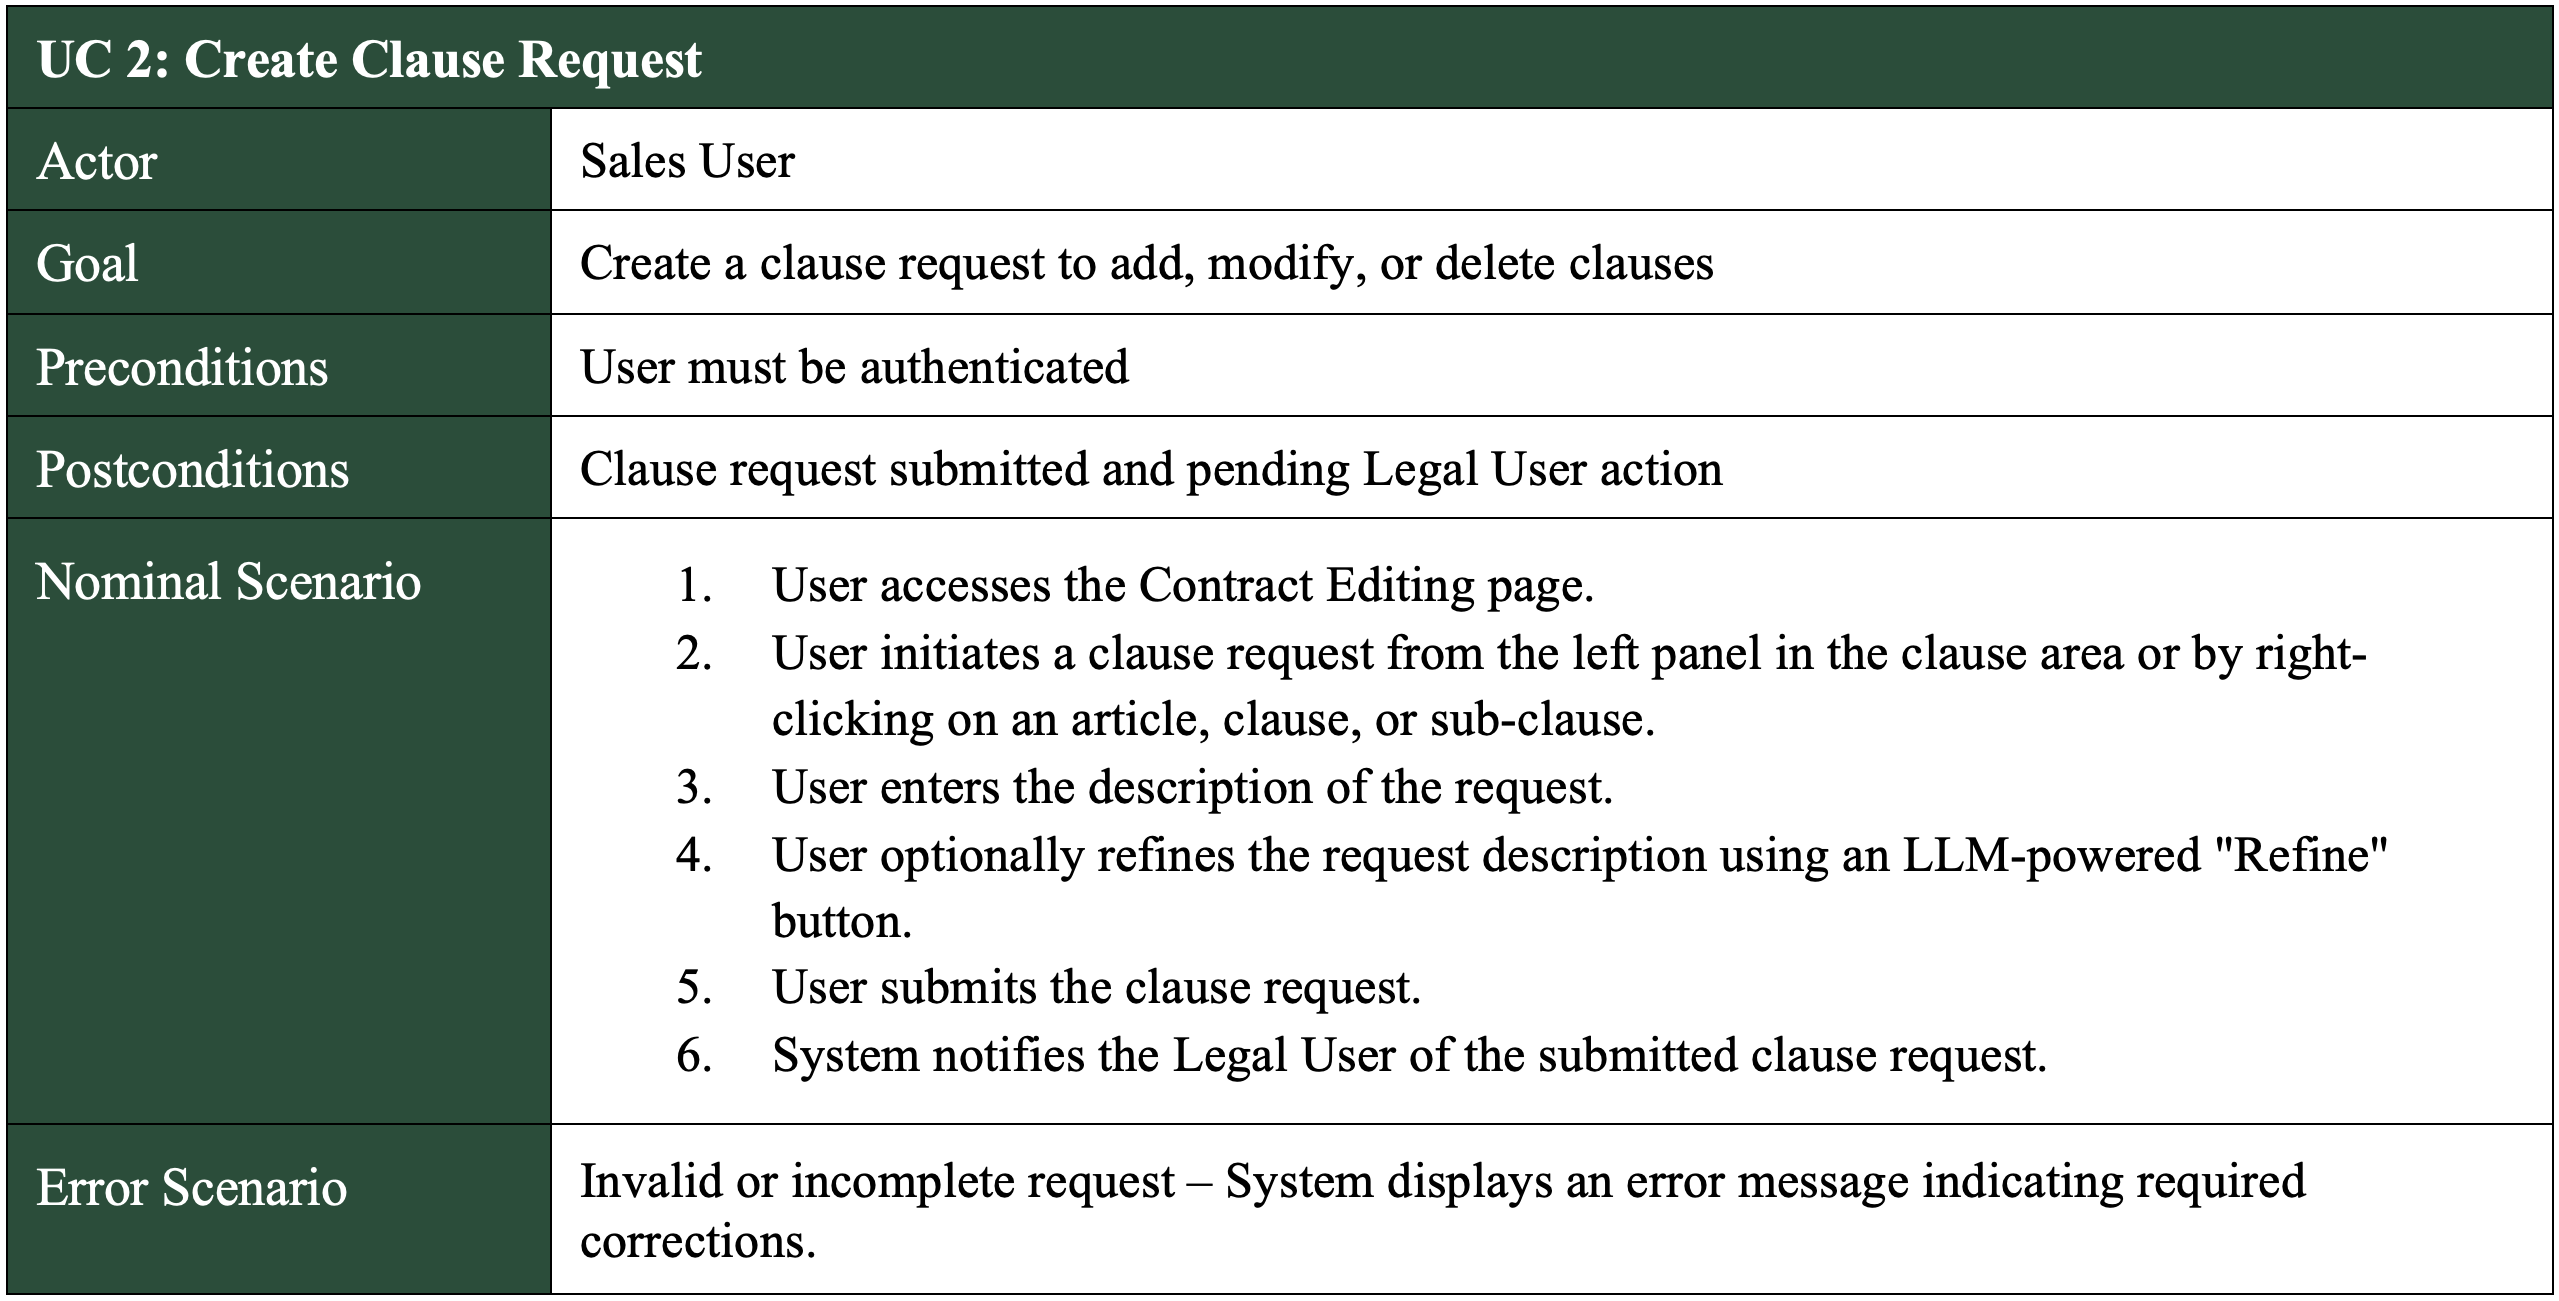
\includegraphics[width=1\textwidth]{Images/Create Clause Request Use Case.png}
    \captionof{table}{Textual Description of Use Case: Create Clause Request}
    \label{tab:create_clause_request_use_case}
\end{center}

\vspace{0.3cm}

\textbf{Textual Description of Use Case: Review Contract}\vspace{-0.3cm}

\begin{center}
    \centering
    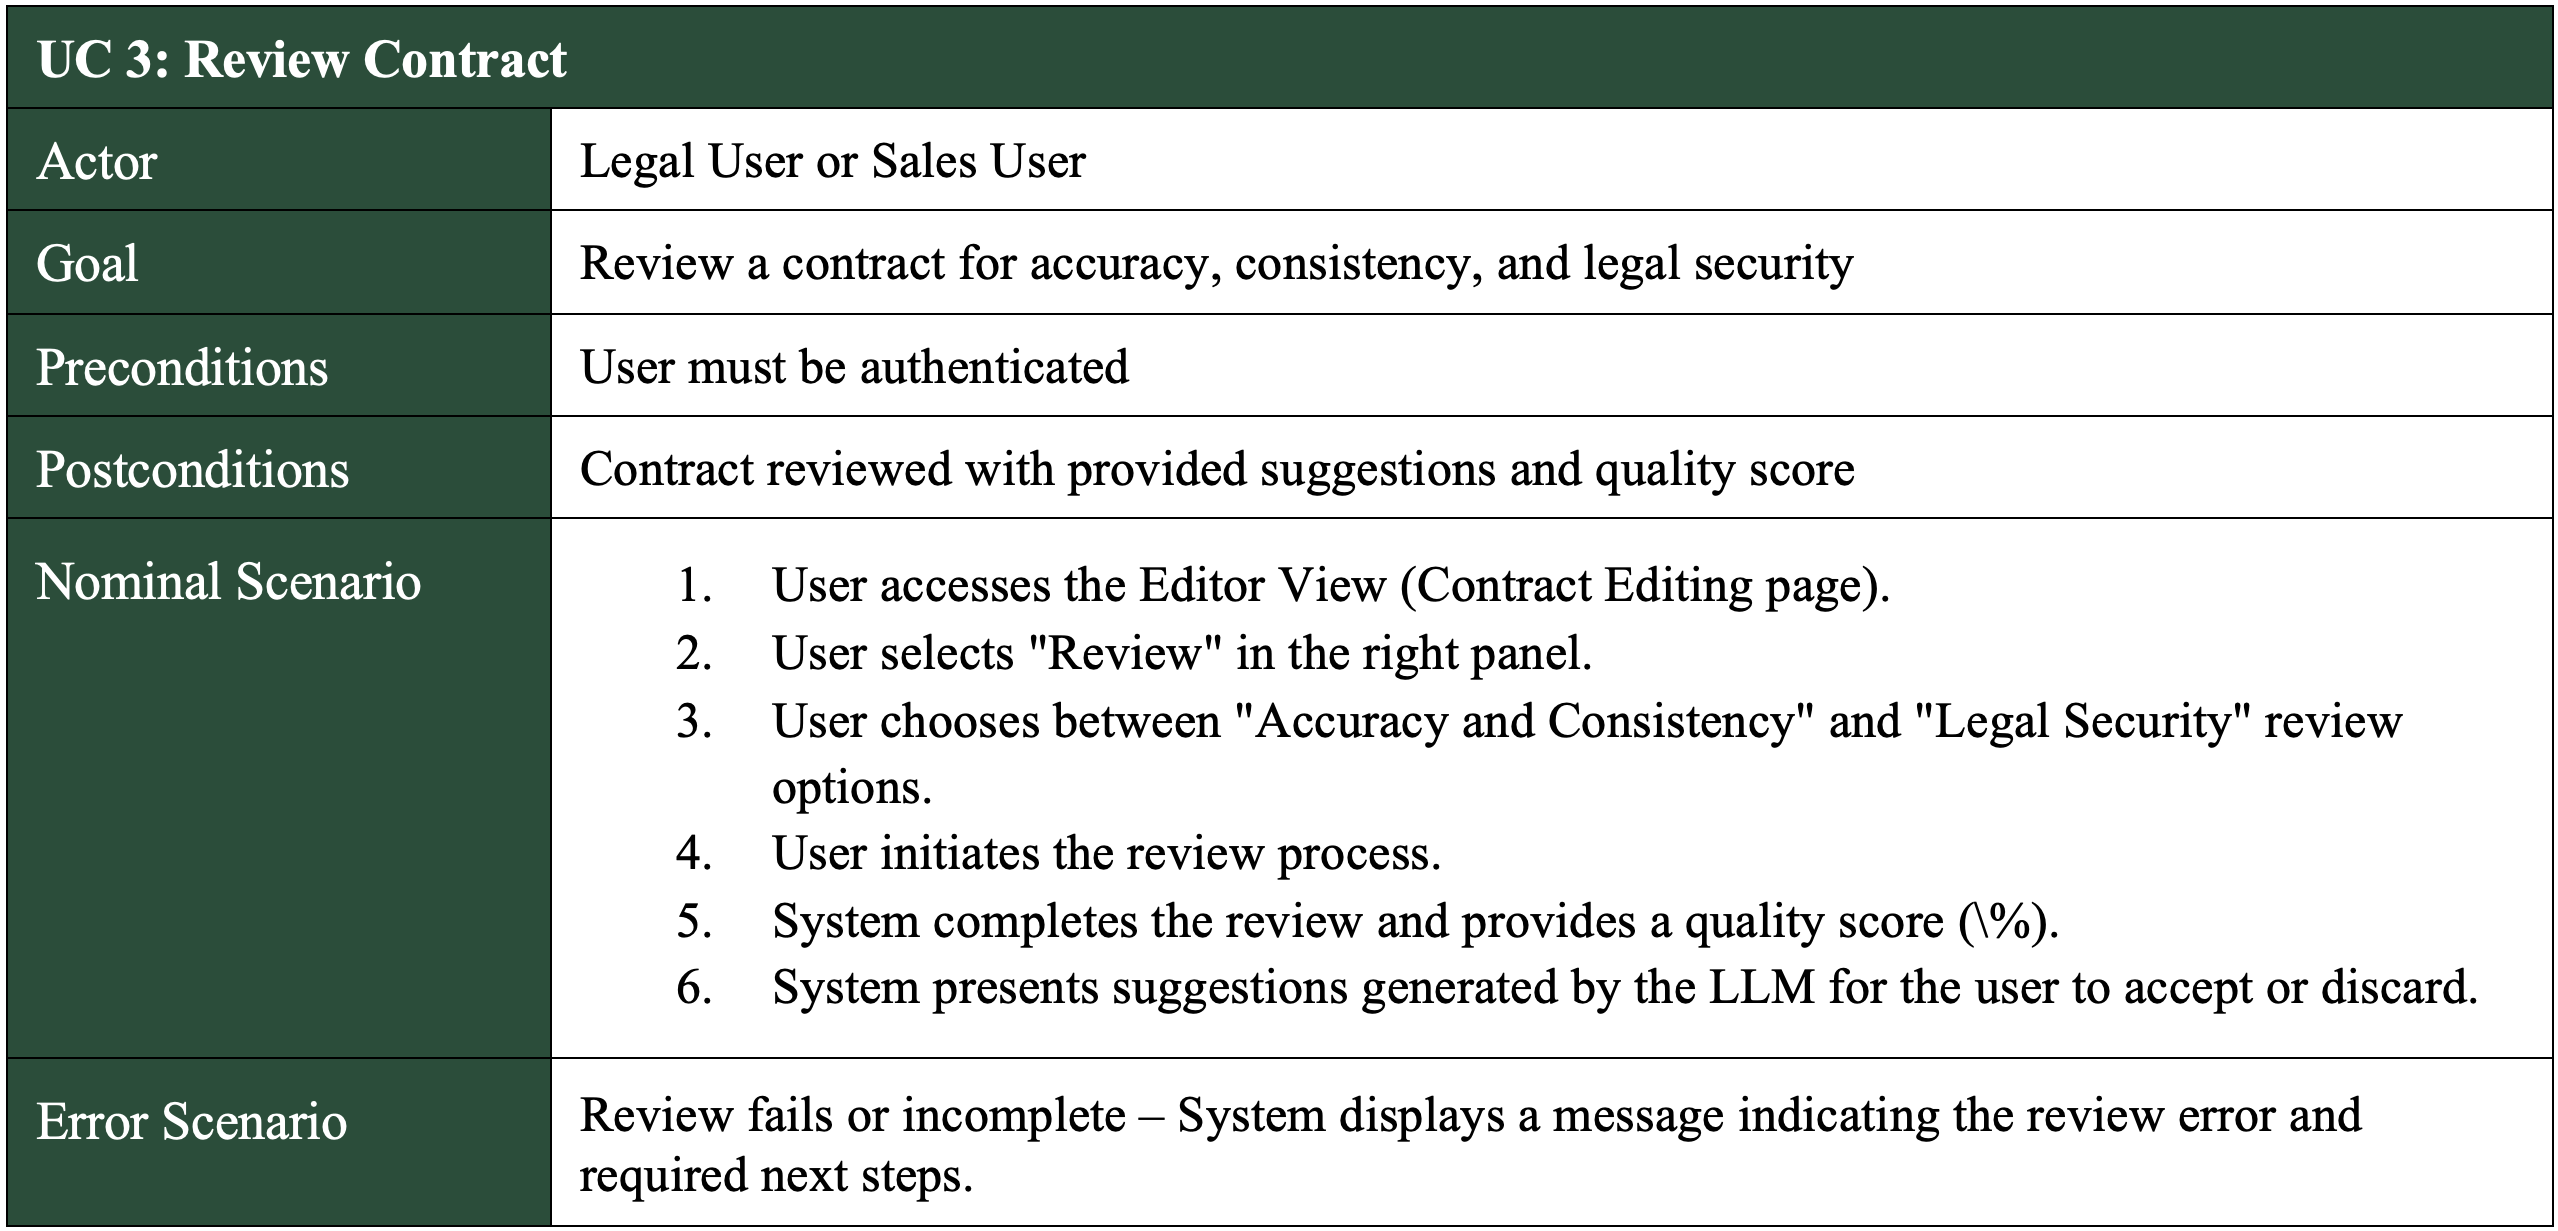
\includegraphics[width=1\textwidth]{Images/Review Contract Use Case.png}
    \captionof{table}{Textual Description of Use Case: Review Contract}
    \label{tab:review_contract_use_case}
\end{center}

% Analysis Sequence Diagram
\subsection{Analysis Sequence Diagram}

\begin{center}
    \centering
    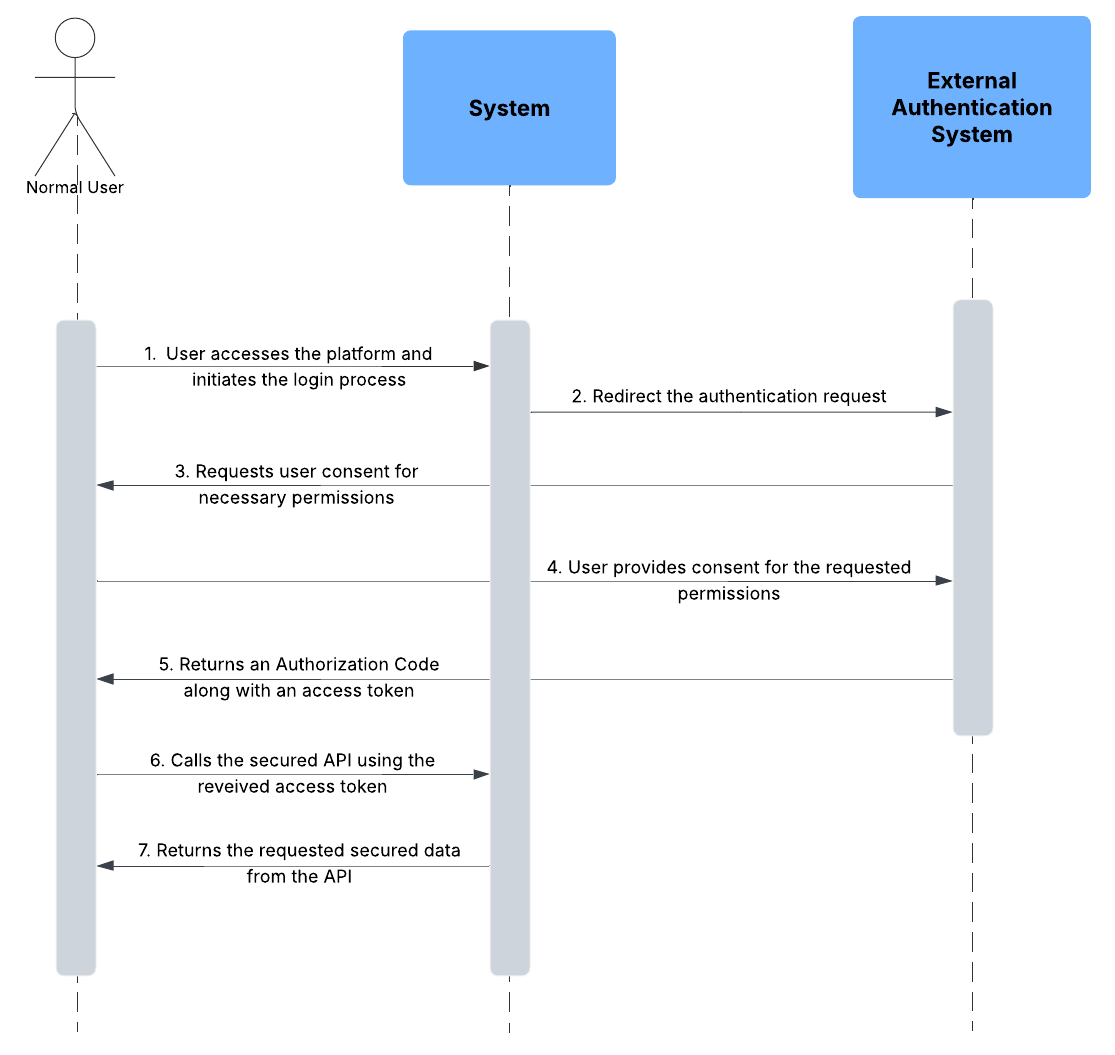
\includegraphics[width=1\textwidth]{Images/Analysis Sequence Diagram.png}
    \captionof{figure}{Analysis Sequence Diagram}
    \label{fig:analysis_sequence_diagram}
\end{center}

The diagram presented above outlines the interaction flow between a normal user intending to authenticate, the main system, and an external authentication system. Initially, the user accesses the platform and clicks on the login button, which prompts the system to redirect the authentication request to the external authentication system. The external authentication system then requests user consent for specific permissions. Upon granting consent by the user, the authentication system issues an authorization code along with an access token back to the system. Finally, the system utilizes this access token to securely call the API and retrieve the requested secured data.

% Constraints and Assumptions
\subsection{Constraints and Assumptions}
To clearly delineate the operational environment and development boundaries, the following constraints and assumptions have been identified:

\textbf{Constraints:}
\begin{itemize}
    \item \textbf{Enterprise Security Compliance}: The system must strictly comply with the organization’s security policies, standards, and regulatory frameworks, ensuring the protection and confidentiality of sensitive contractual and user information.
    \item \textbf{Infrastructure Compatibility}:All technical solutions must be compatible with existing enterprise systems, particularly Azure-based services such as Azure Kubernetes Service (AKS), Azure Entra ID, and Azure PostgreSQL, to ensure seamless integration and minimize disruptions.
    \item \textbf{Cost Efficiency}:The platform must be developed and operated within the allocated budget constraints, adhering to the capacity planning forecasts to optimize resource utilization and cost-effectiveness.
\end{itemize}

\textbf{Assumptions:}
\begin{itemize}
    \item \textbf{Data Availability and Quality}: It is assumed that structured and high-quality data is consistently available from internal sources and third-party integrations to ensure effective AI-driven decision-making.
    \item \textbf{Reliable Cloud Infrastructure}: It is assumed that the Azure cloud infrastructure provides continuous, high-performance service with minimal downtime, ensuring uninterrupted user experiences and workflows.
    \item \textbf{Stable Internet Connectivity}: It is assumed that end users have stable and continuous internet connectivity, enabling consistent access to cloud-hosted services.
    \item \textbf{User Proficiency}: Users are assumed to have a basic level of digital proficiency, enabling them to interact effectively with the intuitive yet sophisticated interfaces provided by the system.
    \item \textbf{Stakeholder Collaboration}: Continuous engagement from all stakeholders, including legal experts, technical teams, and business users, is expected to ensure alignment and smooth progression throughout the project’s lifecycle.
\end{itemize}

% Conclusion
\section{Conclusion}
This chapter detailed the technical rationale behind the project’s approach and identified key enabling technologies. It also defined the system requirements that guide the platform’s architecture, which will be examined in the following chapter.